% ========== CHAPTER 3: SYSTEM DESIGN ==========
% Symphony: An AI-First Development Environment
% Graduation Project - Restructured Chapter
% Team: AMR MUHMAED FATHY, MOHAMED, MAHMOUD, MOSTAFA, SALMA
% Institution: BENHA UNIVERSITY - BFCAI

% \chapter{SYSTEM DESIGN}
% \label{ch:system-design}

% MANUAL FIGURE NUMBERING FOR CHAPTER 3
% Override automatic numbering to ensure figures are always 3.x
\setcounter{chapter}{3}
\setcounter{figure}{0}
\setcounter{table}{0}

\vspace{11cm}

% Chapter Cover
% ========== CHAPTER 3 COVER: SYSTEM DESIGN ==========
% Creative and elegant chapter introduction with sophisticated visual elements
% Following the established 4-element pattern

\vspace{2cm}

% 1. BIG CHAPTER NUMBER in content-reflective shape (diamond for design/architecture)
\begin{center}
\begin{tikzpicture}
    % Diamond shape for design/architectural content
    \fill[brandAccent!15] (0,2.2) -- (2.2,0) -- (0,-2.2) -- (-2.2,0) -- cycle;
    % Chapter number
    \node[font=\fontsize{80}{80}\selectfont\bfseries, color=brandAccent] at (0,0) {3};
\end{tikzpicture}
\end{center}

\vspace{0cm}

% 2. CHAPTER TOPIC with elegant typography
\begin{center}
{\fontsize{28}{32}\selectfont\textcolor{brandPrimary}{\textit{System Design}}}
\end{center}

\vspace{0.2cm}

% 3. NICE SEPARATOR with decorative elements
\begin{center}
\textcolor{brandAccent}{
\rule{2cm}{0.8pt} \quad
\raisebox{-0.2ex}{\Large$\bullet$} \quad
\rule{4cm}{0.8pt} \quad
\raisebox{-0.2ex}{\Large$\bullet$} \quad
\rule{2cm}{0.8pt}
}
\end{center}

\vspace{0cm}

% 4. "THIS CHAPTER EXPLORES" content box
\begin{tcolorbox}[
    enhanced,
    colback=white,
    colframe=brandAccent!40,
    boxrule=1pt,
    arc=12pt,
    drop shadow={brandAccent!20},
    left=1.5cm,
    right=1.5cm,
    top=1.0cm,
    bottom=1.0cm,
    before upper={\parindent0pt}
]
\begin{center}
{\Large\textbf{\textcolor{brandAccent}{This chapter explores}}}
\end{center}

\vspace{0.8cm}

\begin{itemize}[leftmargin=1.2cm, itemsep=0.4cm, label={\textcolor{brandAccent}{$\triangleright$}}]
    \item {\large The overall architectural vision and design philosophy behind Symphony}
    \item {\large Core system components including the microkernel and orchestration engine}
    \item {\large The Dual Ensemble Architecture separating infrastructure from community extensions}
    \item {\large How the extension system enables unlimited customization and community innovation}
    \item {\large The orchestration system design for coordinating multiple AI agents}
    \item {\large Data flow patterns, system integration, and user interface design principles}
    \item {\large Generic primitives and protocol support for extensibility}
\end{itemize}
\end{tcolorbox}

\clearpage


% Section 3.1: System Architecture Overview
% Section 3.3: System Architecture Overview

\section{3.3 System Architecture Overview}
\label{sec:architecture-overview}
\addcontentsline{toc}{section}{3.3 System Architecture Overview}

\lettrine{T}{his section} presents Symphony's architectural foundation based on the Harmonic Hexagonal Actor Architecture (H²A²) and the multi-phase bootstrap process. The architecture emphasizes separation of concerns, fault isolation, and intelligent orchestration for AI-first development.

\subsection*{3.3.1 H²A² Architecture and Design Philosophy}
\addcontentsline{toc}{subsection}{3.3.1 H²A² Architecture and Design Philosophy}

Symphony's architecture embraces a microkernel design philosophy prioritizing modularity and extensibility. The foundation rests on the Harmonic Hexagonal Actor Architecture (H²A²), combining hexagonal architecture with actor-based concurrency models.

The H²A² Architecture establishes clear boundaries between domain logic and infrastructure adapters. The Domain Core maintains workflow definitions, extension policies, and orchestration logic, operating independently through well-defined port interfaces. The architecture consists of four key layers:

\textbf{Layer 1a: Domain Core Components}

The Domain Core contains three essential components: OrchestrationEngine for workflow scheduling, WorkflowDefinitions for templates and validation, and ExtensionPolicies for security rules. These define system behavior independent of implementation details.


\begin{figure}[H]
\centering
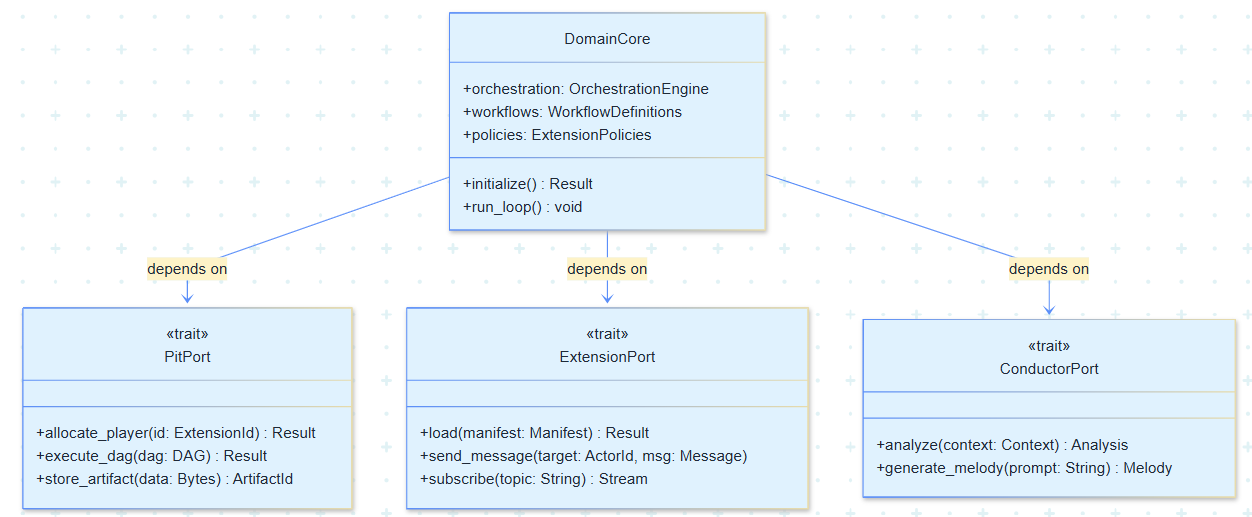
\includegraphics[width=1.15\textwidth]{images/diagrams/class_diagram/seperate_1_h2a2_architecture_domain_adapters/H²A² Architecture Part1 part1.png}
\caption{H²A² Architecture - Domain Core Components}
\label{fig:3.6a-h2a2-domain-components}
\end{figure}

\clearpage
\textbf{Layer 1b: Port Interfaces}

The Domain Core depends on abstract port interfaces that define contracts for external interactions. PitPort handles player allocation, DAG execution, and artifact storage. ExtensionPort manages extension loading, messaging, and topic subscriptions. ConductorPort provides context analysis and melody generation capabilities. TextEditingPort handles text insertion, deletion, and editing operations. These interfaces enable the core to remain independent of concrete implementations as illustrated in Figure 3.3.

\begin{figure}[H]
\centering
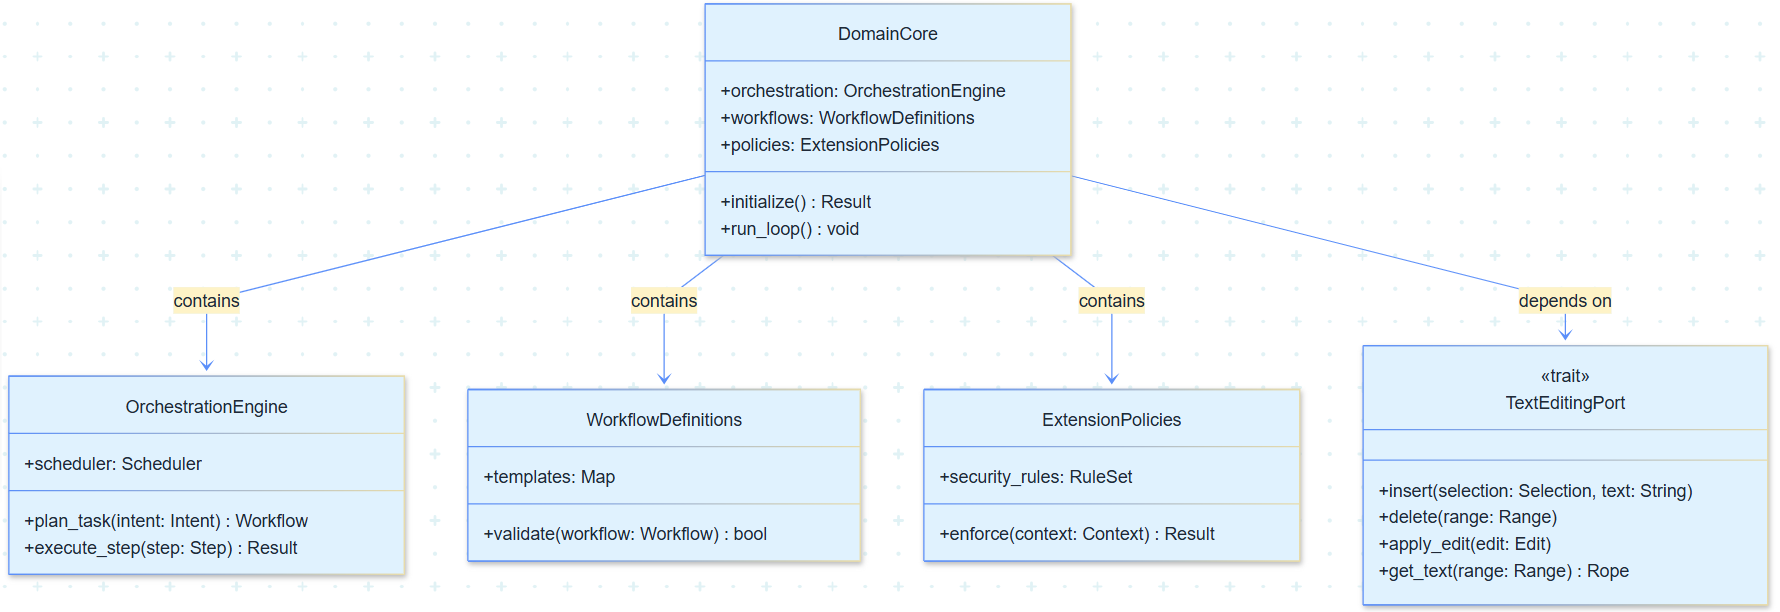
\includegraphics[width=1.15\textwidth]{images/diagrams/class_diagram/seperate_1_h2a2_architecture_domain_adapters/H²A² Architecture Part1 part2.png}
\caption{H²A² Architecture - Port Interfaces Layer}
\label{fig:3.7-h2a2-ports}
\end{figure}

\textbf{Layer 2: Extension and Orchestration Adapters}

The second layer handles extension management and AI orchestration. The ActorExtensionAdapter manages The Grand Stage actor-based extension system, coordinating instruments, operators, and motifs through the actor registry and supervisor strategy. The ConductorAdapter bridges communication with the Python-based reinforcement learning model, enabling intelligent workflow generation through context analysis and melody generation capabilities as illustrated in Figure 3.4.

\begin{figure}[H]
\centering
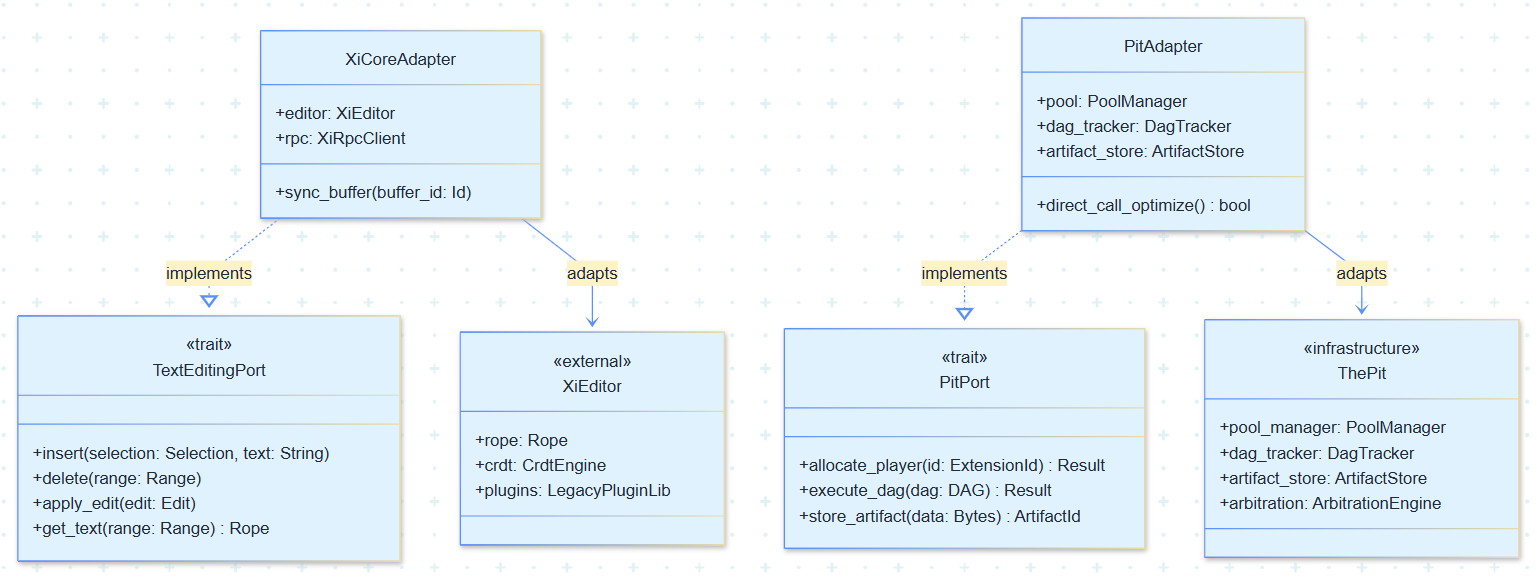
\includegraphics[width=0.95\textwidth]{images/diagrams/class_diagram/seperate_1_h2a2_architecture_domain_adapters/H²A² Architecture Part2.png}
\caption{H²A² Architecture - Extension and Orchestration Adapters Layer}
\label{fig:3.8-h2a2-orchestration}
\end{figure}

\textbf{Layer 3: Domain Core and Port Interfaces}

The third layer represents the Domain Core with its abstract port interfaces. The core contains the OrchestrationEngine, WorkflowDefinitions, and ExtensionPolicies that define system behavior at a conceptual level. Port interfaces (TextEditingPort, PitPort, ExtensionPort, ConductorPort) define contracts for external interactions without specifying implementation details. This separation enables the system to remain adaptable to changing requirements without requiring fundamental redesigns as illustrated in Figure 3.5.

\begin{figure}[H]
\centering
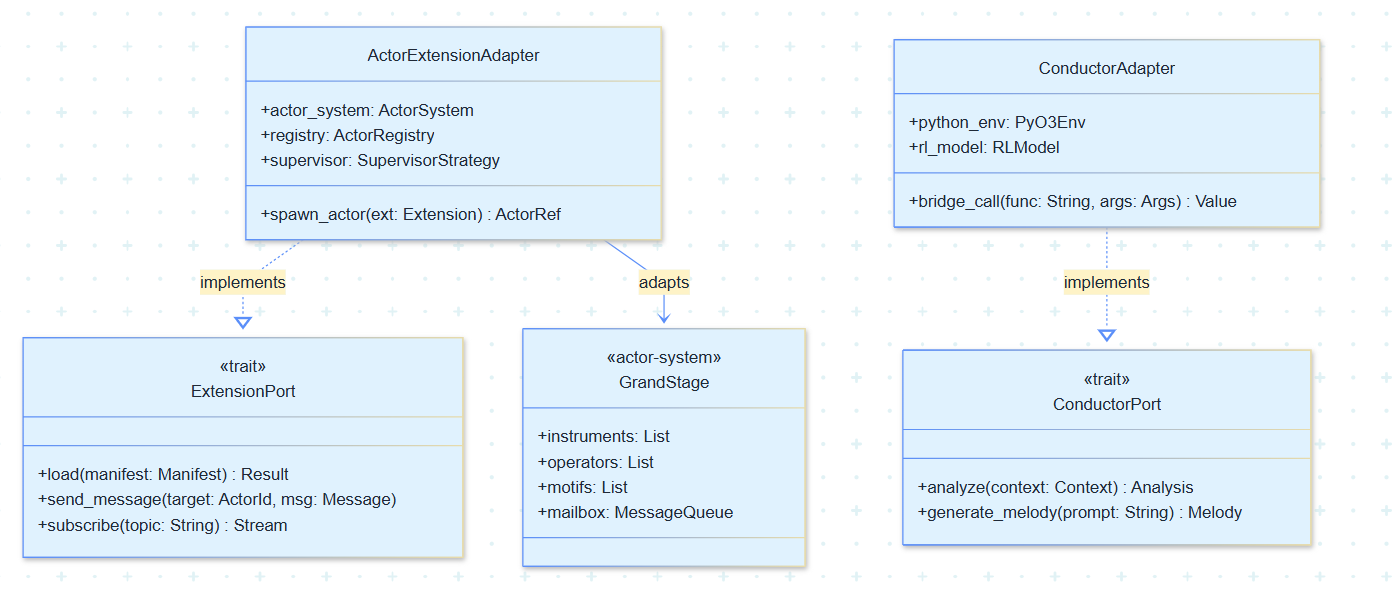
\includegraphics[width=1.15\textwidth]{images/diagrams/class_diagram/seperate_1_h2a2_architecture_domain_adapters/H²A² Architecture Part3.png}
\caption{H²A² Architecture - Domain Core and Port Interfaces Layer}
\label{fig:3.9-h2a2-domain}
\end{figure}

% The microkernel philosophy keeps the core system minimal while delegating specialized functionality to extensions. This contrasts with monolithic IDE architectures that bundle extensive functionality into the core, resulting in bloated applications with slow startup times. Symphony's microkernel contains only essential primitives for orchestration, extension management, and system coordination, while all other capabilities are provided through dynamically loaded extensions.

\clearpage
\subsection*{3.3.2 System Bootstrap and Initialization}
\addcontentsline{toc}{subsection}{3.3.2 System Bootstrap and Initialization}

Symphony's initialization follows a carefully orchestrated bootstrap process through five distinct phases as shown in Figure 3.6, each building upon previous phases with dependency satisfaction and health verification at each stage:

\begin{compactlist}
    \item \textbf{Foundation Phase}: Establishes type system, loads configuration, initializes core orchestration engine
    \item \textbf{IPC Phase}: Sets up inter-process communication infrastructure for extension communication
    \item \textbf{Pit Phase}: Initializes high-performance in-process components (Pool Manager, DAG Tracker, Artifact Store, Arbitration Engine, Stale Manager)
    \item \textbf{Conductor Phase}: Loads Python-based RL model, establishes PyO3 bindings for Rust-Python communication
    \item \textbf{UI Phase}: Brings up user interface, establishes WebSocket connections, performs comprehensive health checks
\end{compactlist}

The architectural design incorporates sophisticated error handling and recovery mechanisms. If any bootstrap phase encounters errors, the system automatically initiates rollback procedures, cleanly shutting down successfully initialized components and returning to a safe state. This rollback capability extends to runtime operations, where component failures are isolated to prevent cascading failures.

The H²A² Architecture's separation of concerns provides significant benefits: new capabilities can be added through additional adapters without modifying the Domain Core, infrastructure components can be upgraded by providing new adapter implementations satisfying existing port interfaces, and comprehensive testing is facilitated through isolated Domain Core testing with mock implementations and adapter testing against port interface contracts.

\begin{figure}[H]
\centering
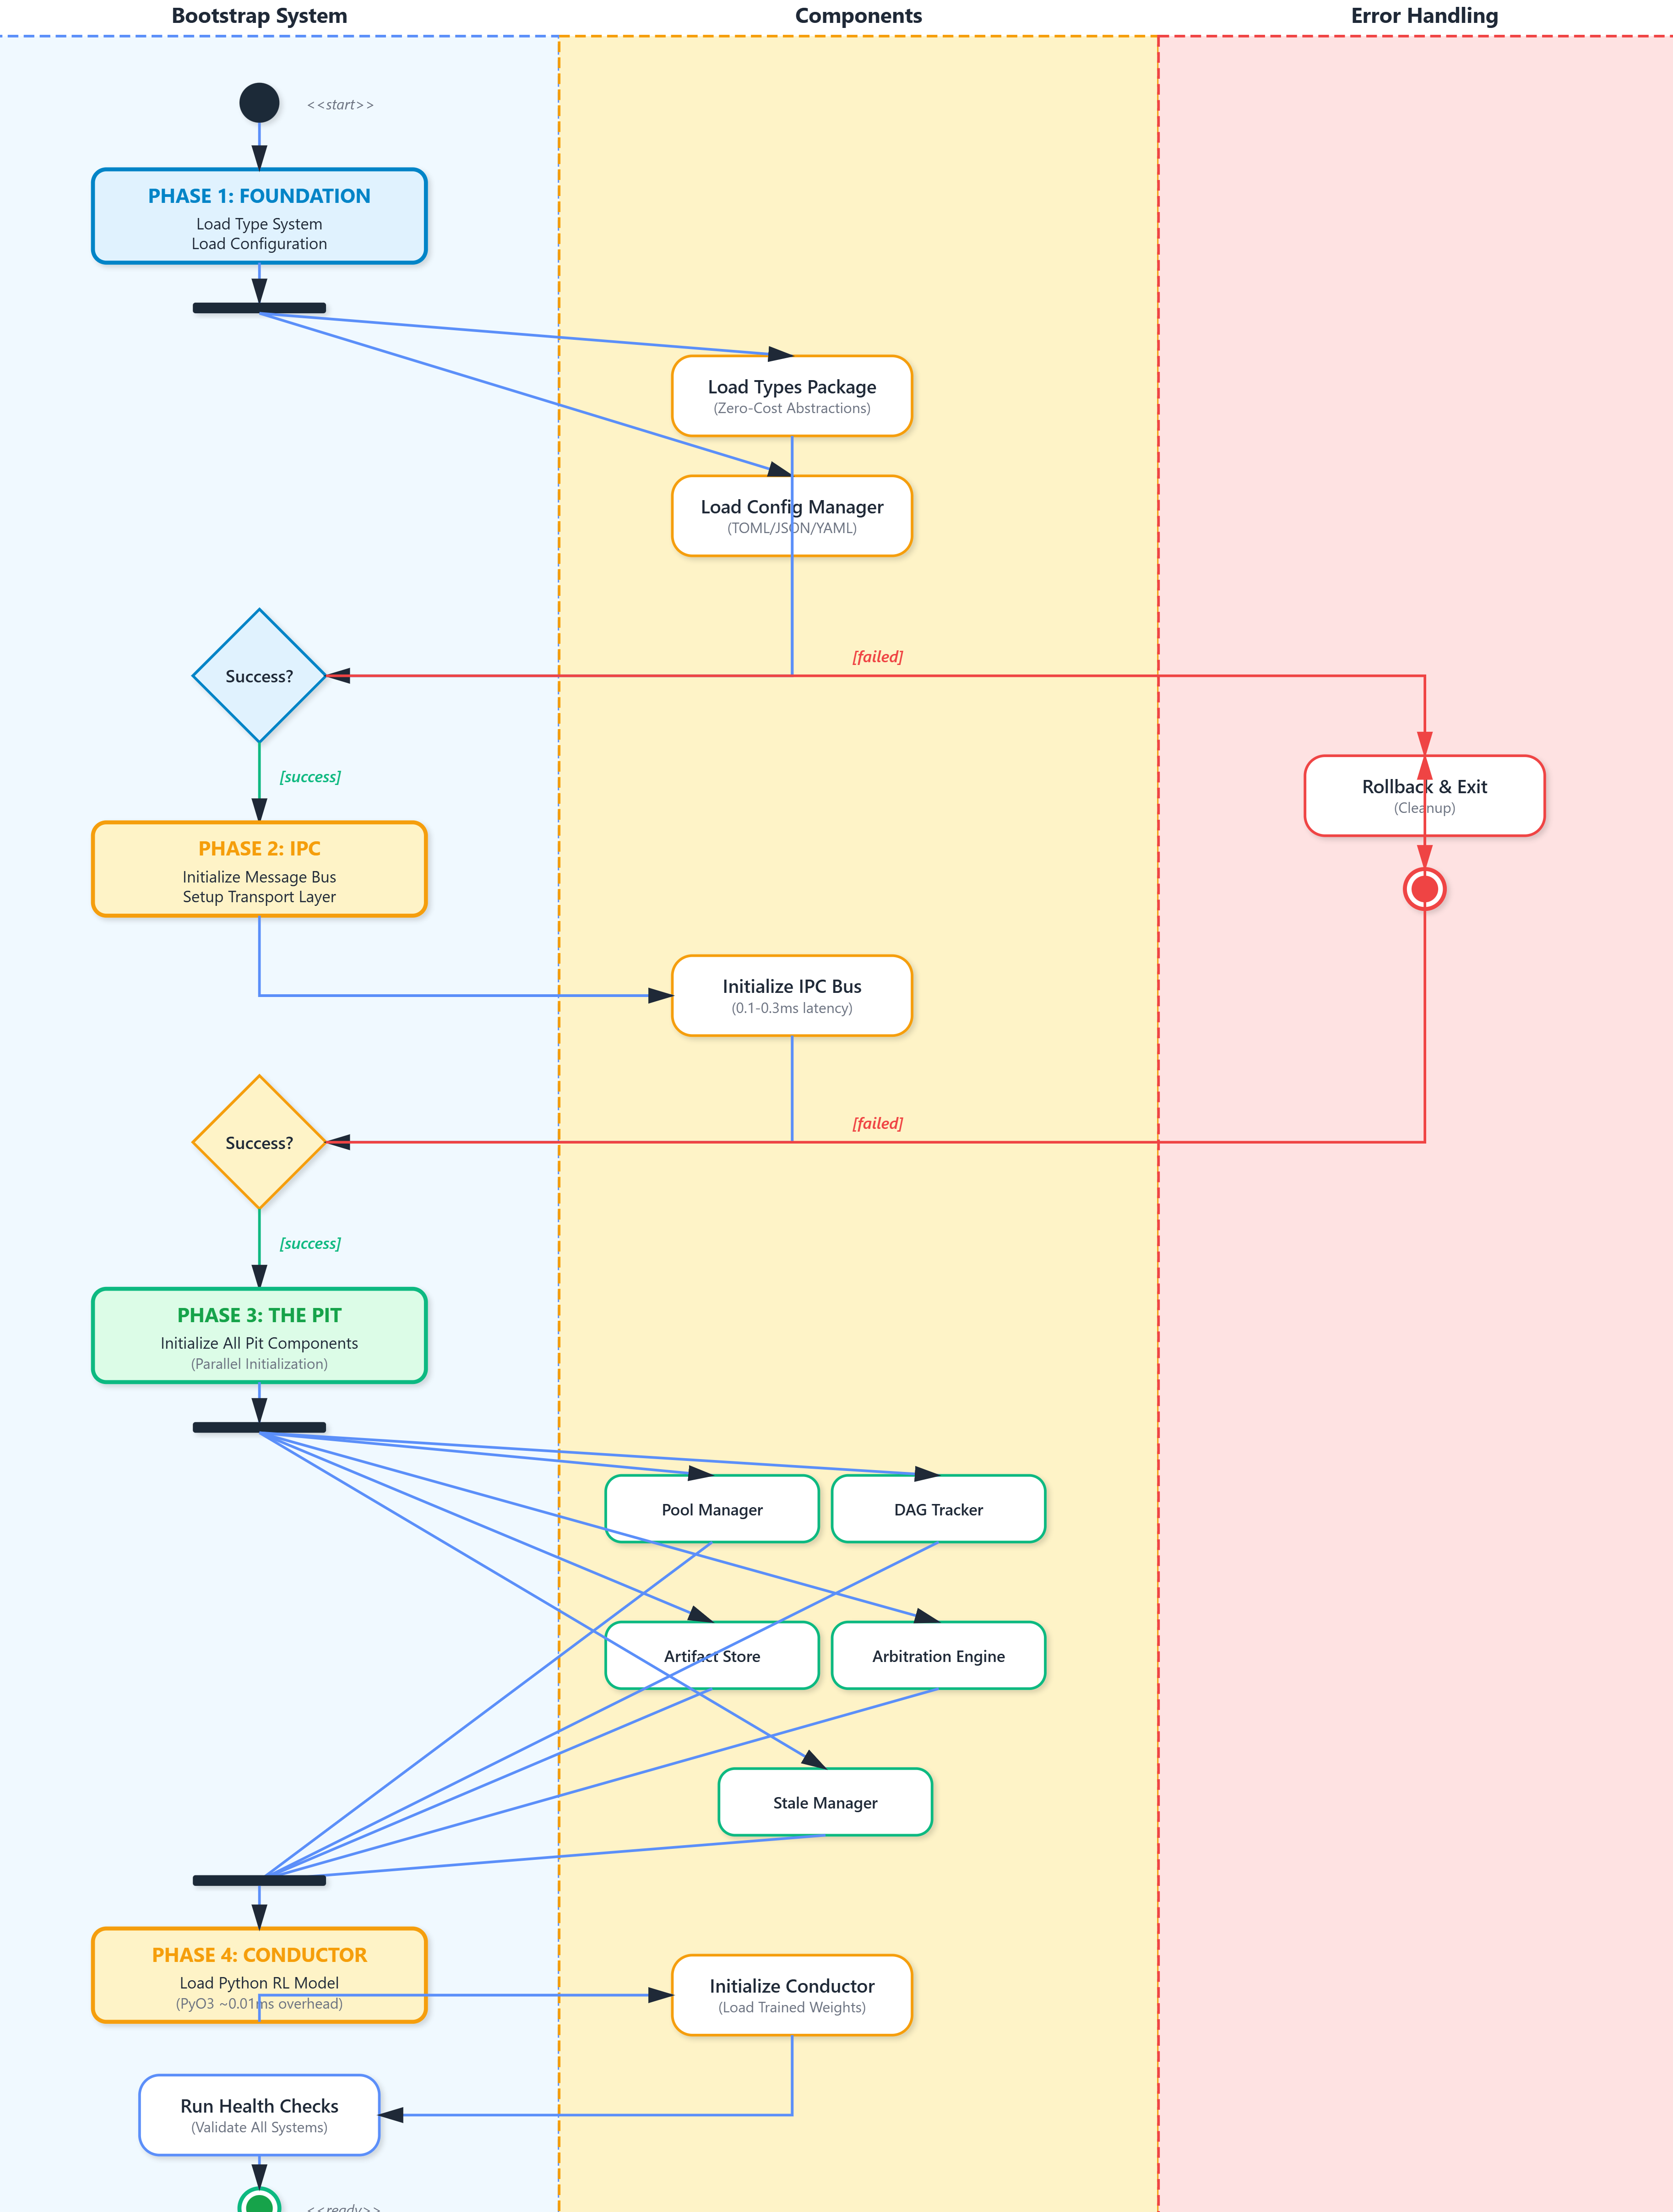
\includegraphics[width=1.25\textwidth]{images/diagrams/activity_diagram/symphony-system-bootstrap.png}
\caption{System Bootstrap Process}
\label{fig:3.10}
\end{figure}




% Section 3.2: Core System Components
% Section 3.5: Core System Components

\section{3.5 Core System Components}
\label{sec:core-components}
\addcontentsline{toc}{section}{3.5 Core System Components}

\lettrine{T}{he} minimal core philosophy guides Symphony's design through a systematic selection methodology. Components are included in the core only if they meet specific criteria: universally required by all development workflows, performance-critical where extension boundaries would introduce prohibitive overhead, security-sensitive requiring deep system integration, or foundational as building blocks for extensions. This "extension-first mindset" ensures that the core remains truly minimal while maintaining full functionality through the extension ecosystem.

The benefits of this approach include startup times under one second compared to three to eight seconds for traditional environments, memory footprint below 150 megabytes compared to over 500 megabytes for feature-rich alternatives, and approximately 40 percent faster startup with 25 percent lower memory usage while maintaining equivalent functionality through extensions.


\subsection*{3.5.1 Six Essential Core Components}

Based on the selection methodology, six essential components form Symphony's minimal core:

\begin{description}[leftmargin=4cm,labelwidth=3.5cm]
    \item[\textbf{Text Processing Engine}] Fundamental text manipulation capabilities with extension interfaces for advanced features
    \item[\textbf{Project Navigation}] Essential file system interaction with extensible visualization and management
    \item[\textbf{Syntax Analysis}] Core language processing with pluggable grammar and semantic analysis
    \item[\textbf{Configuration Management}] Centralized preference system with extension integration capabilities
    \item[\textbf{System Integration}] Native platform interaction with secure extension access patterns
    \item[\textbf{Extension Orchestration}] Dynamic loading and coordination system enabling unlimited functionality expansion
\end{description}

Everything beyond these six components is delegated to extensions, allowing users to customize their environment precisely to their needs without carrying unnecessary overhead.

\subsection*{3.5.2 Domain Core and Orchestration}

The Domain Core serves as the central coordination system, managing workflow definitions, enforcing extension policies, and coordinating execution of multi-step processes involving multiple AI agents and tools. The OrchestrationEngine within the Domain Core analyzes developer requests, breaks them into constituent tasks, determines appropriate operation sequences, and coordinates execution across multiple extensions and AI models.


\subsection*{3.5.3 Intelligence as Extension Principle}

Symphony treats intelligence as an extension rather than embedding AI capabilities directly into the core. This architectural decision provides several advantages: AI models can be updated without modifying the core system, multiple AI providers and models can operate simultaneously, and different AI capabilities can be selected for different tasks based on specific requirements and performance characteristics. The Conductor, which contains the reinforcement learning model for workflow orchestration, exemplifies this principle by operating as a Python-based extension that communicates with the core through well-defined interfaces.

\subsection*{3.5.4 Generic Primitives Foundation}

The core provides generic primitives that establish the foundation for all extension functionality. These primitives include basic operations for process management, inter-process communication, resource allocation, and event notification. By providing these capabilities as generic primitives rather than specialized features, the core enables extensions to compose complex behaviors from simple building blocks while ensuring robust, well-tested fundamental operations.


% Section 3.3: Dual Ensemble Architecture
% Section 3.6: Dual Ensemble Architecture
\clearpage
\section{3.6 Dual Ensemble Architecture}
\label{sec:dual-ensemble}
\addcontentsline{toc}{section}{3.6 Dual Ensemble Architecture}

\lettrine{T}{he} Dual Ensemble Architecture provides two distinct execution environments optimized for different performance and safety requirements. This dual-layer approach enables ultra-low-latency execution for trusted operations while maintaining robust isolation for community-developed extensions.

\subsection*{3.6.1 The Pit: In-Process Execution}

The Pit constitutes the high-performance in-process execution environment for trusted infrastructure extensions. Five core components operate within The Pit: Pool Manager, DAG Tracker, Artifact Store, Arbitration Engine, and Stale Manager. Extensions execute within the same process as the core system, enabling direct function calls and shared memory access with nanosecond-level latencies.

\textbf{Institutional Memory and Resource Management Components}

The first architectural view of The Pit focuses on institutional memory, lifecycle management, and resource arbitration capabilities. As illustrated in Figure~\ref{fig:pit-core-memory-arbitration}, the PitCore serves as the central registry managing all in-process extensions through registration, unregistration, and retrieval operations. The PitCore maintains references to five critical infrastructure components, with three highlighted in this view.

The ArtifactStore provides Symphony's institutional memory system, storing artifacts with content-addressable hashing and Tantivy-based full-text indexing. Each artifact contains versioned data, metadata, quality scores, and timestamps, enabling efficient retrieval, search, and deduplication. The quality scoring mechanism ensures high-value artifacts receive priority in storage and retrieval operations.

The StaleManager handles artifact lifecycle transitions across storage tiers based on access patterns and age. The lifecycle management system defines three stages: SSD storage for frequently accessed artifacts (1-7 days), HDD storage for moderately accessed content (8-30 days), and cloud archival for long-term retention (30+ days). The StaleManager monitors artifact usage, triggers transitions between lifecycle stages, and performs cleanup operations to optimize storage utilization.

The ArbitrationEngine resolves resource conflicts when multiple workflows compete for limited resources. The engine maintains fairness policies, resolves conflicts through intelligent resource allocation strategies, applies fairness algorithms to prevent resource starvation, and prioritizes tasks based on urgency, importance, and historical patterns. This ensures optimal resource utilization while maintaining system responsiveness.

\begin{figure}[H]
\centering
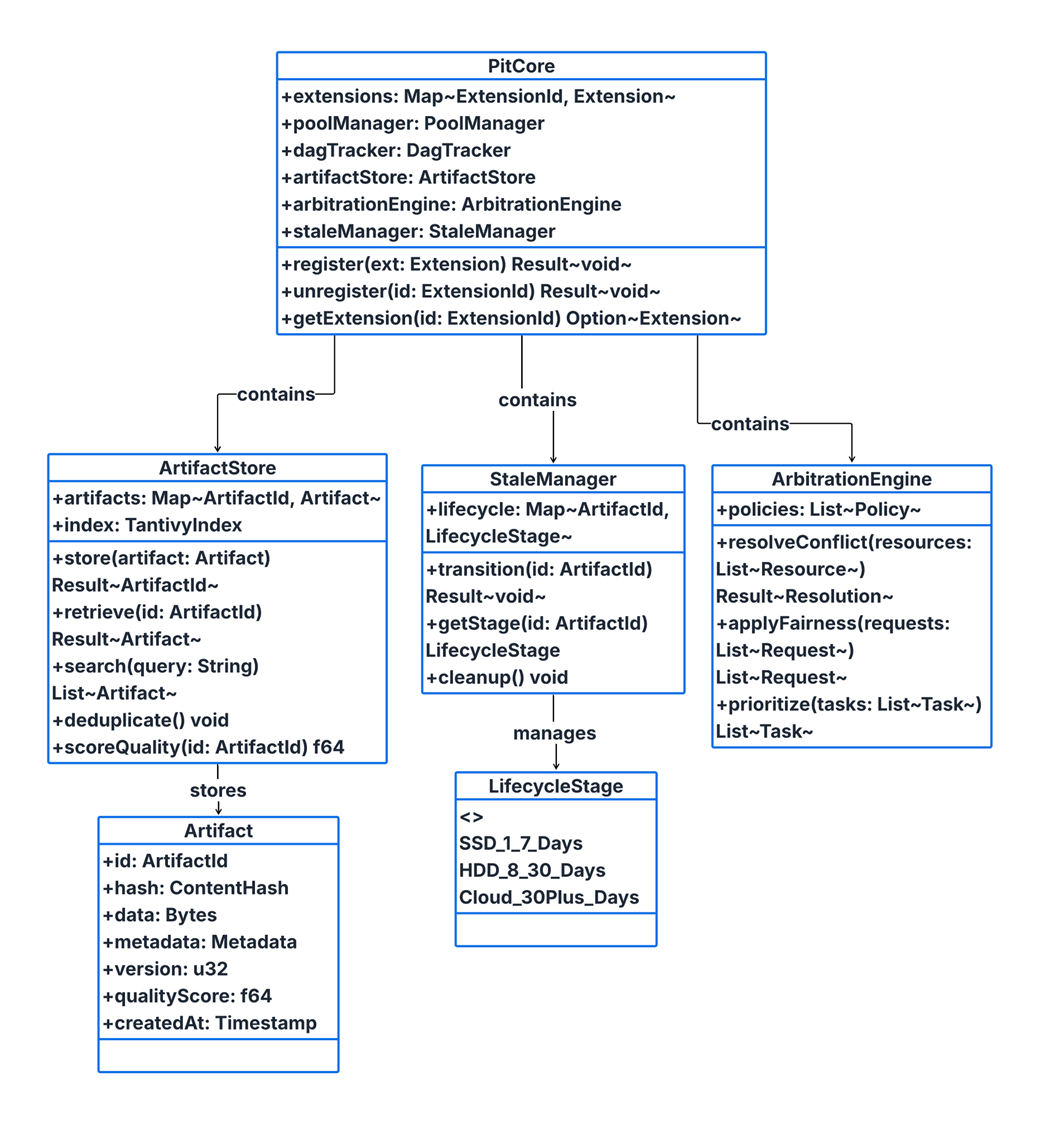
\includegraphics[width=1.0\textwidth]{images/diagrams/class_diagram/PitCore/PitCore1.png}
\caption{The Pit Architecture - Institutional Memory and Resource Management Components}
\label{fig:pit-core-memory-arbitration}
\end{figure}

\clearpage
\textbf{Workflow Execution and AI Model Management Components}

The second architectural view, shown in Figure~\ref{fig:pit-core-workflow-pool}, illustrates The Pit's workflow orchestration and AI model lifecycle management capabilities. The PitCore continues to serve as the central coordination point, now highlighting the DagTracker and PoolManager components that enable intelligent workflow execution and model resource optimization.

The DagTracker manages workflow execution through directed acyclic graph (DAG) representation and coordination. The tracker maintains a registry of workflows mapped by MelodyId, executes melodies by coordinating node execution according to dependency constraints, performs topological sorting to determine optimal execution order, supports parallel execution of independent nodes to maximize throughput, and provides checkpoint and resume capabilities for long-running workflows. Each DAG node represents a workflow step with defined inputs, outputs, extension identifiers, and parameter configurations.

The PoolManager handles AI model lifecycle management with intelligent resource optimization. The manager maintains a registry of players (AI models and extensions) mapped by ExtensionId, tracking their current state through the PlayerState enumeration (Unloaded, Loading, Warming, Ready, Active). The LRU cache mechanism optimizes memory utilization by tracking recently used models and evicting least-recently-used entries when memory pressure increases. The predictive pre-warming capability analyzes usage patterns to anticipate which models will be needed next, proactively loading them before requests arrive to minimize perceived latency. The allocation and deallocation methods manage player lifecycle, while state queries enable the system to make informed scheduling decisions.

Together, these components enable The Pit to achieve microsecond-level operation latencies through in-process execution, shared memory access, and zero-copy data transfer between components. This performance profile makes The Pit essential for Symphony's real-time AI orchestration and workflow execution capabilities.

\begin{figure}[H]
\centering
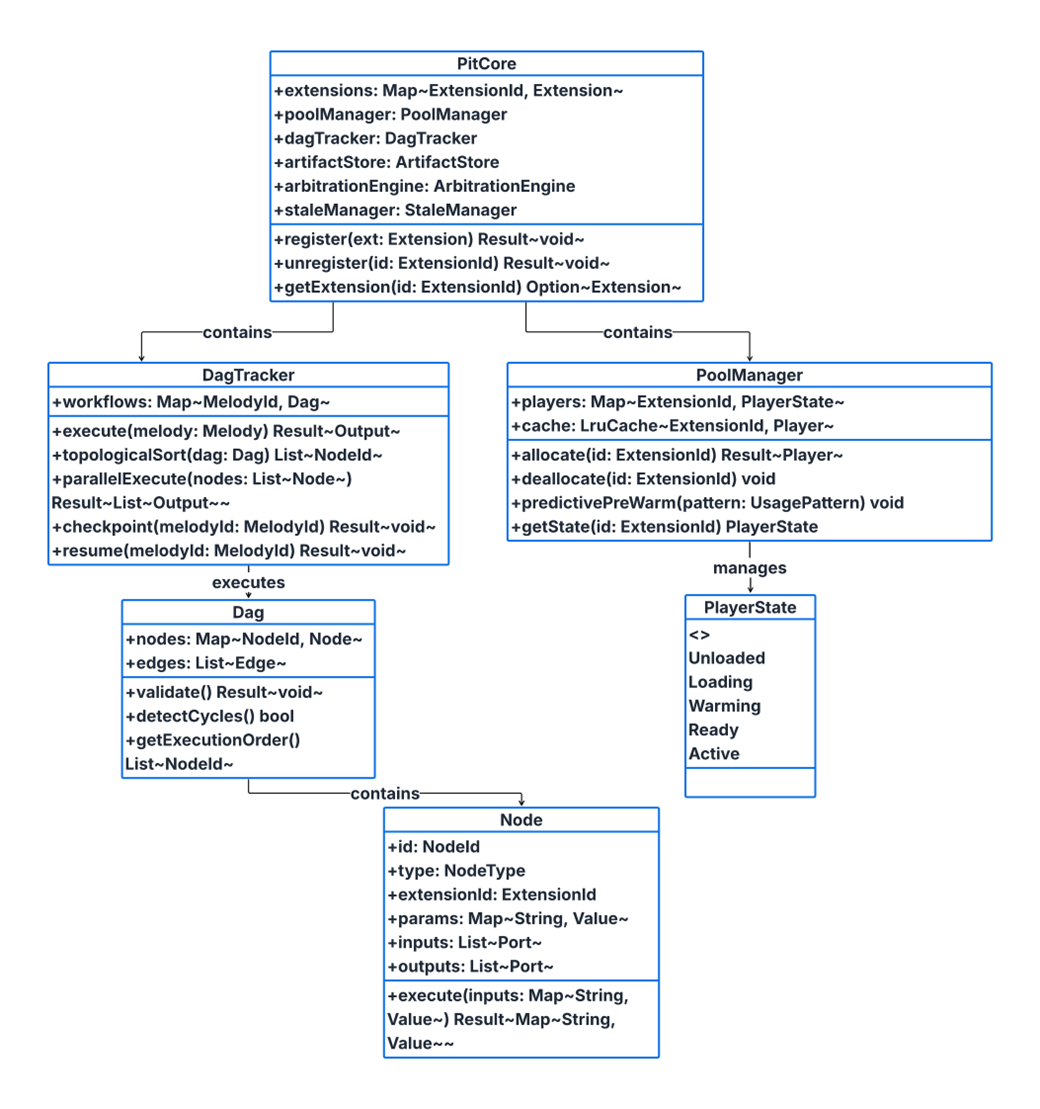
\includegraphics[width=1.0\textwidth]{images/diagrams/class_diagram/PitCore/PitCore2.png}
\caption{The Pit Architecture - Workflow Execution and AI Model Management Components}
\label{fig:pit-core-workflow-pool}
\end{figure}

\clearpage
\subsection*{3.6.2 The Grand Stage: Out-of-Process Execution}

The Grand Stage provides the out-of-process execution environment for community-developed extensions requiring strong isolation guarantees. Extensions execute in separate processes with well-defined communication channels, ensuring that bugs or malicious behavior cannot compromise system stability or security. The Grand Stage employs an actor-based concurrency model where each extension runs as an independent actor with its own mailbox for receiving messages.

While The Grand Stage incurs additional overhead from inter-process communication resulting in latencies measured in fractions of a millisecond, this overhead remains imperceptible to users for most operations and provides essential protection against risks of running untrusted code.

\subsection*{3.6.3 Security and Trust Framework}

Symphony implements a multi-layered security approach protecting users while enabling innovation as shown in ~\ref{Multi-Layer Security Framework}:

\begin{table}[H]
\caption{Multi-Layer Security Framework}
\label{Multi-Layer Security Framework}
\centering
\begin{tabular}{@{}lll@{}}
\toprule
\textbf{Security Layer} & \textbf{Mechanism} & \textbf{Protection} \\
\midrule
Sandboxed Execution & Process isolation & Fault containment \\
Permission System & Capability-based access & Resource protection \\
Code Review & Automated scanning & Vulnerability prevention \\
Runtime Monitoring & Behavioral analysis & Anomaly detection \\
\bottomrule
\end{tabular}
\end{table}

The capability-based security framework provides fine-grained control over extension permissions through minimal privilege principle, dynamic capability adjustment based on behavior and trust levels, capability inheritance for controlled privilege escalation, and immediate revocation mechanisms in response to security threats.

The trust-based security model adapts to extension behavior over time through behavioral trust scoring with continuous assessment of patterns, community trust metrics integrating user feedback and ratings, graduated trust levels providing progressive capability access based on demonstrated reliability, and trust decay mechanisms for inactive or problematic extensions.

\subsection*{3.6.4 Player Registration System}

Extensions can register as Players to participate in Conductor orchestration, gaining enhanced capabilities and visibility. The Player system provides:

\begin{compactlist}
    \item Intelligent extension selection based on workflow requirements
    \item Performance monitoring and quality assurance
    \item Enhanced integration with Symphony's AI orchestration
    \item Elevated marketplace visibility and user trust
\end{compactlist}

Players commit to governance policies including performance standards and security compliance, with continuous SLA monitoring ensuring adherence. The Conductor chooses optimal Players for tasks based on capabilities, performance characteristics, and trust levels.

\subsection*{3.6.5 Execution Strategy Selection}

The system determines execution environment based on multiple factors including trust level, performance requirements, resource usage patterns, and security considerations. Infrastructure extensions that are part of Symphony's core distribution execute in The Pit for optimal performance, while community-developed extensions and experimental features execute on The Grand Stage for isolation and protection.


% Section 3.4: Extension System Design
% Section 3.7: Extension System Design
\clearpage
\section{3.7 Extension System Design}
\label{sec:extension-system}
\addcontentsline{toc}{section}{3.7 Extension System Design}

\lettrine{T}{he} extension system represents the primary mechanism through which Symphony achieves unlimited customization and adaptation to diverse development scenarios. The system delegates specialized functionality to extensions that can be independently developed, tested, and deployed, enabling rapid evolution through community contributions while maintaining a stable core.

\subsection*{3.7.1 Extension Categories: Instruments, Operators, and Motifs}

Symphony defines three distinct extension categories, each serving different purposes with appropriate execution environments and integration patterns:

\begin{description}[leftmargin=3cm,labelwidth=2.5cm]
    \item[\textbf{Instruments}] AI and ML models providing intelligence capabilities such as code generation, analysis, and transformation
    \item[\textbf{Operators}] Workflow utilities and data processing functions handling file manipulation, transformation, and external tool integration
    \item[\textbf{Motifs}] User interface enhancements providing custom visualizations, specialized editors, and interaction patterns
\end{description}

This categorization enables the system to apply appropriate policies and optimizations based on extension type. Instruments integrate with Symphony's AI orchestration system, Operators provide deterministic operations complementing probabilistic AI models, and Motifs integrate with the web-based user interface leveraging modern web technologies as shown in ~\ref{Extension Type Execution Optimization}.

\begin{table}[H]
\caption{Extension Type Execution Optimization}
\label{Extension Type Execution Optimization}
\centering
\begin{tabular}{@{}lll@{}}
\toprule
\textbf{Extension Type} & \textbf{Execution Model} & \textbf{Optimization Focus} \\
\midrule
Instruments & Isolated processes & Resource management, AI model lifecycle \\
Operators & Lightweight containers & Fast startup, minimal overhead \\
Motifs & Web runtime & UI responsiveness, visual performance \\
\bottomrule
\end{tabular}
\end{table}

\clearpage
\subsection*{3.7.2 Orchestra Kit Framework}

The Orchestra Kit provides comprehensive infrastructure for managing the complete extension lifecycle from discovery through installation, loading, activation, and execution. The framework consists of specialized components working together seamlessly, which can be understood through three main groups:

\textbf{Component Group 1: Discovery and Distribution}

The first group handles extension discovery and distribution. The Registry manages metadata for all available extensions, enabling discovery and version management through extension registration, search queries, and version tracking. The Marketplace (The Grand Stage) serves as the distribution platform with browsing capabilities, download management, package uploads, ratings, and reviews. The Installer handles secure deployment with package installation, dependency resolution, signature verification, and rollback capabilities as illustrated in ~\ref{fig:3.12-orchestra-discovery}.

\begin{figure}[H]
\centering
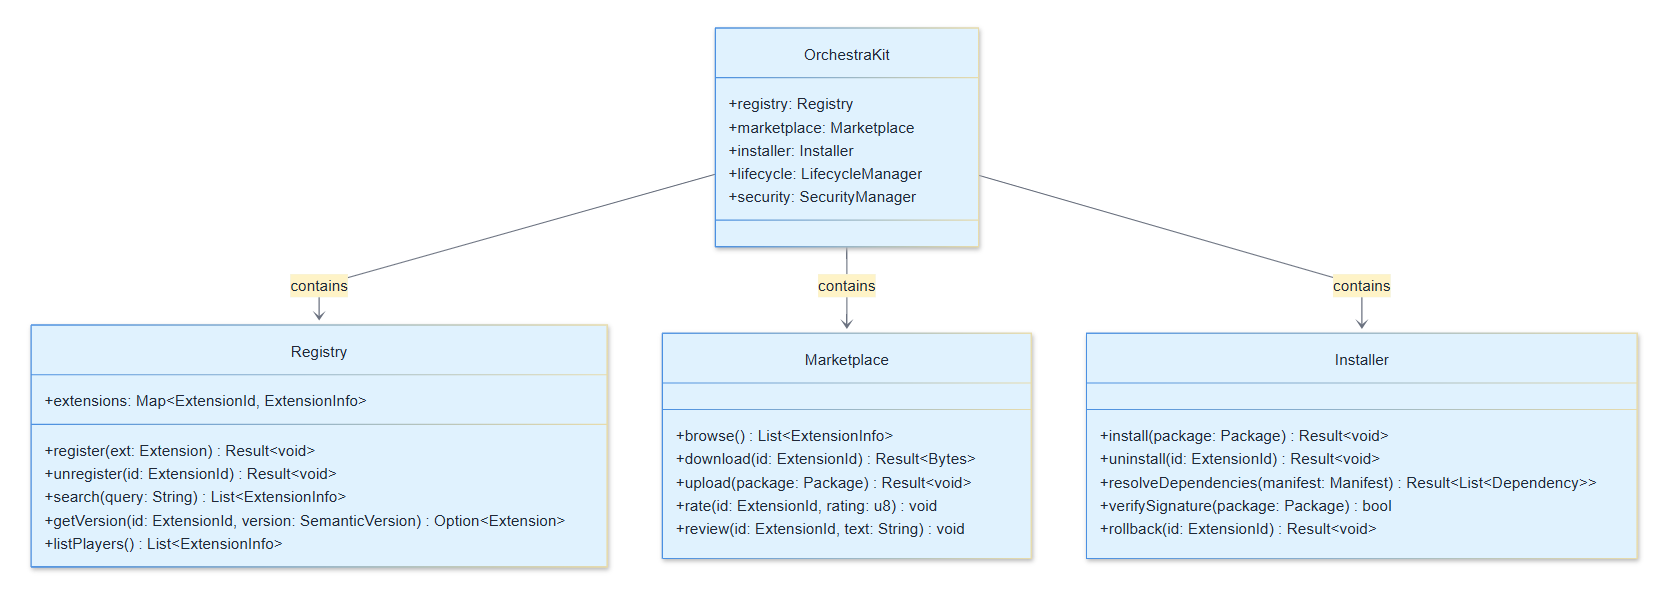
\includegraphics[width=1.15\textwidth]{images/diagrams/class_diagram/seperate_4_orchestra_kit_extension_ecosystem/Orchestra Kit Part1.png}
\caption{Orchestra Kit - Discovery and Distribution Components}
\label{fig:3.12-orchestra-discovery}
\end{figure}

\clearpage
\textbf{Component Group 2: Lifecycle and Security Management}

The second group manages extension lifecycle and security. The LifecycleManager implements the Chambering state machine, tracking extension states (Installed, Loading, Loaded, Activated, Running) and coordinating state transitions. The SecurityManager provides protection through sandboxing for process isolation, permission management for capability-based access control, and resource enforcement. The PermissionManager handles role-based access with permission checking, granting, revoking, and action auditing as illustrated in ~\ref{fig:3.13-orchestra-lifecycle}.

\begin{figure}[H]
\centering
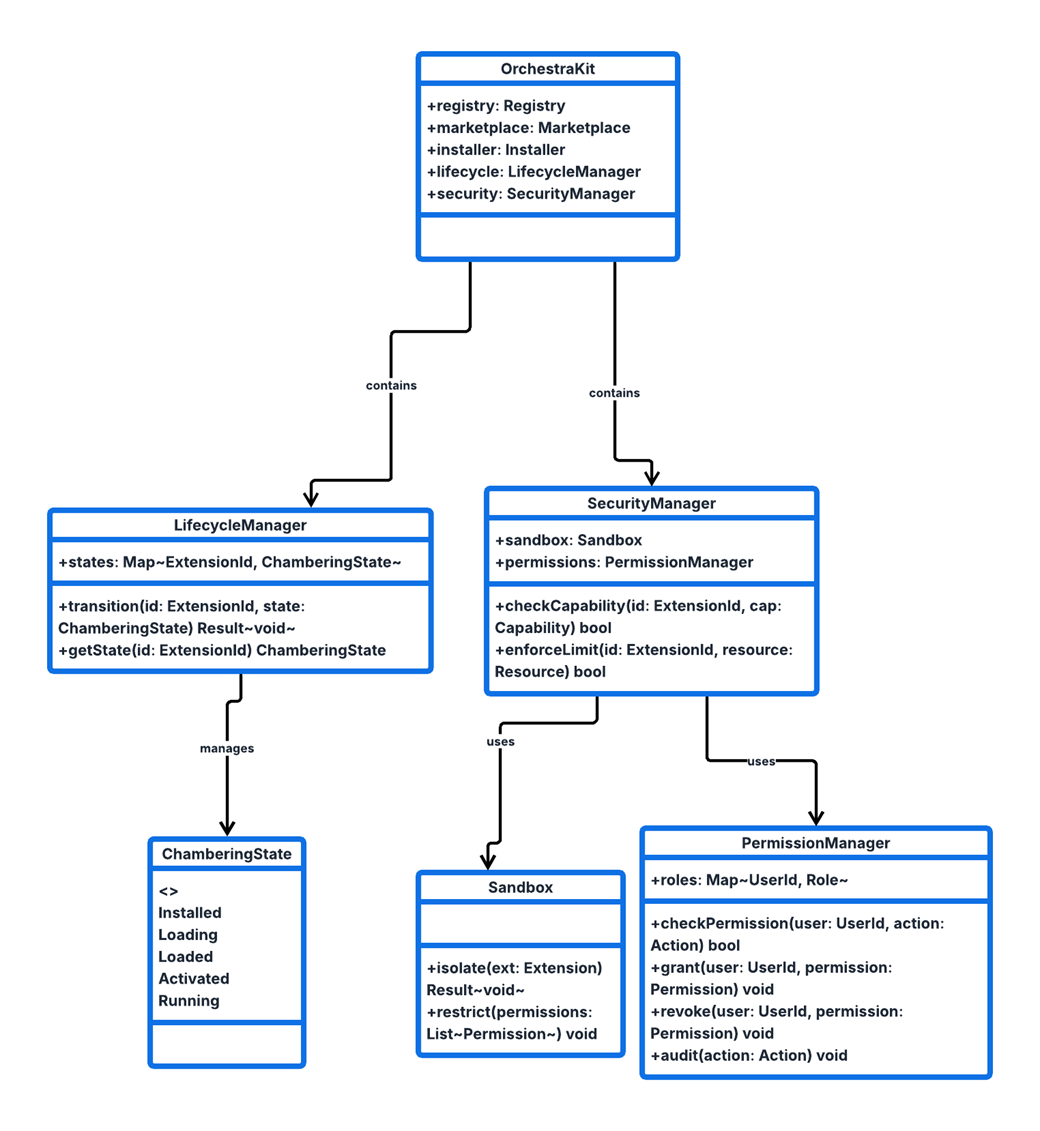
\includegraphics[width=1.15\textwidth]{images/diagrams/class_diagram/seperate_4_orchestra_kit_extension_ecosystem/Orchestra Kit Part2.png}
\caption{Orchestra Kit - Lifecycle and Security Management Components}
\label{fig:3.13-orchestra-lifecycle}
\end{figure}

\clearpage
\textbf{Component Group 3: Development Toolchain}

The third group provides the development toolchain. CaretsCli offers command-line interface for creating new extensions, running tests, publishing to marketplace, and scaffolding from templates. ExtensionSdk provides the development framework with core SDK functionality, testing framework with mocks and fixtures, and metrics collection for performance monitoring. This toolchain supports the complete development workflow from project creation through marketplace publication as illustrated in ~\ref{fig:3.14-orchestra-toolchain}.

\begin{figure}[H]
\centering
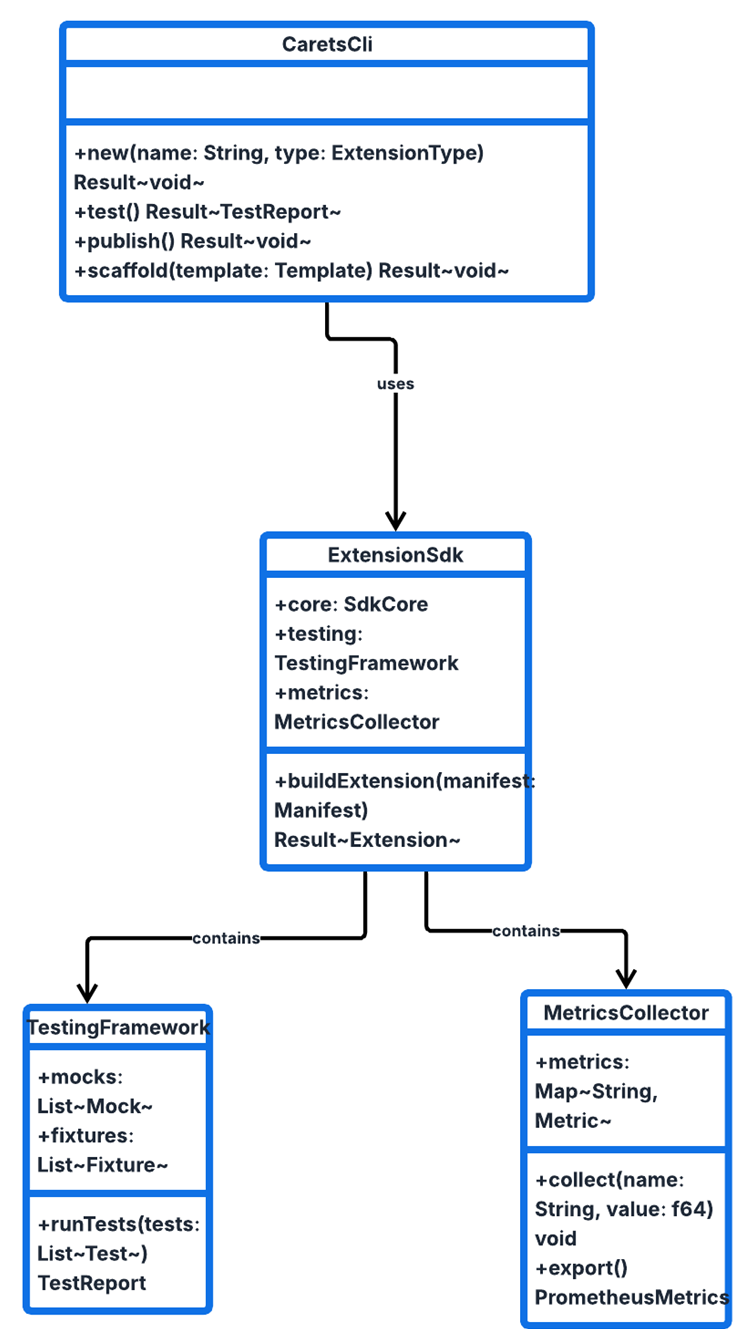
\includegraphics[width=0.95\textwidth]{images/diagrams/class_diagram/seperate_4_orchestra_kit_extension_ecosystem/CaretsCLISDK.png}
\caption{Orchestra Kit - Development Toolchain (Carets CLI and SDK)}
\label{fig:3.14-orchestra-toolchain}
\end{figure}


\subsection*{3.7.3 Extension Lifecycle and Chambering Process}

The extension lifecycle follows a well-defined state machine known as the Chambering process, governing transitions from installation through activation and execution. Extensions progress through distinct states including Installed, Loading, Loaded, Activating, Active, Deactivating, Unloading, and Uninstalled. Each state transition is carefully managed to ensure proper initialization before use and efficient resource management throughout the lifecycle.

The Chambering process ensures that extensions are properly validated before activation, resources are allocated efficiently during loading, and cleanup occurs systematically during unloading. State transitions are atomic operations that either complete successfully or roll back to the previous stable state, preventing partial initialization that could compromise system stability. The state machine governs all possible transitions and ensures that extensions follow the correct lifecycle path as illustrated in ~\ref{fig:3.15-extension-lifecycle}.

\begin{figure}[H]
\centering
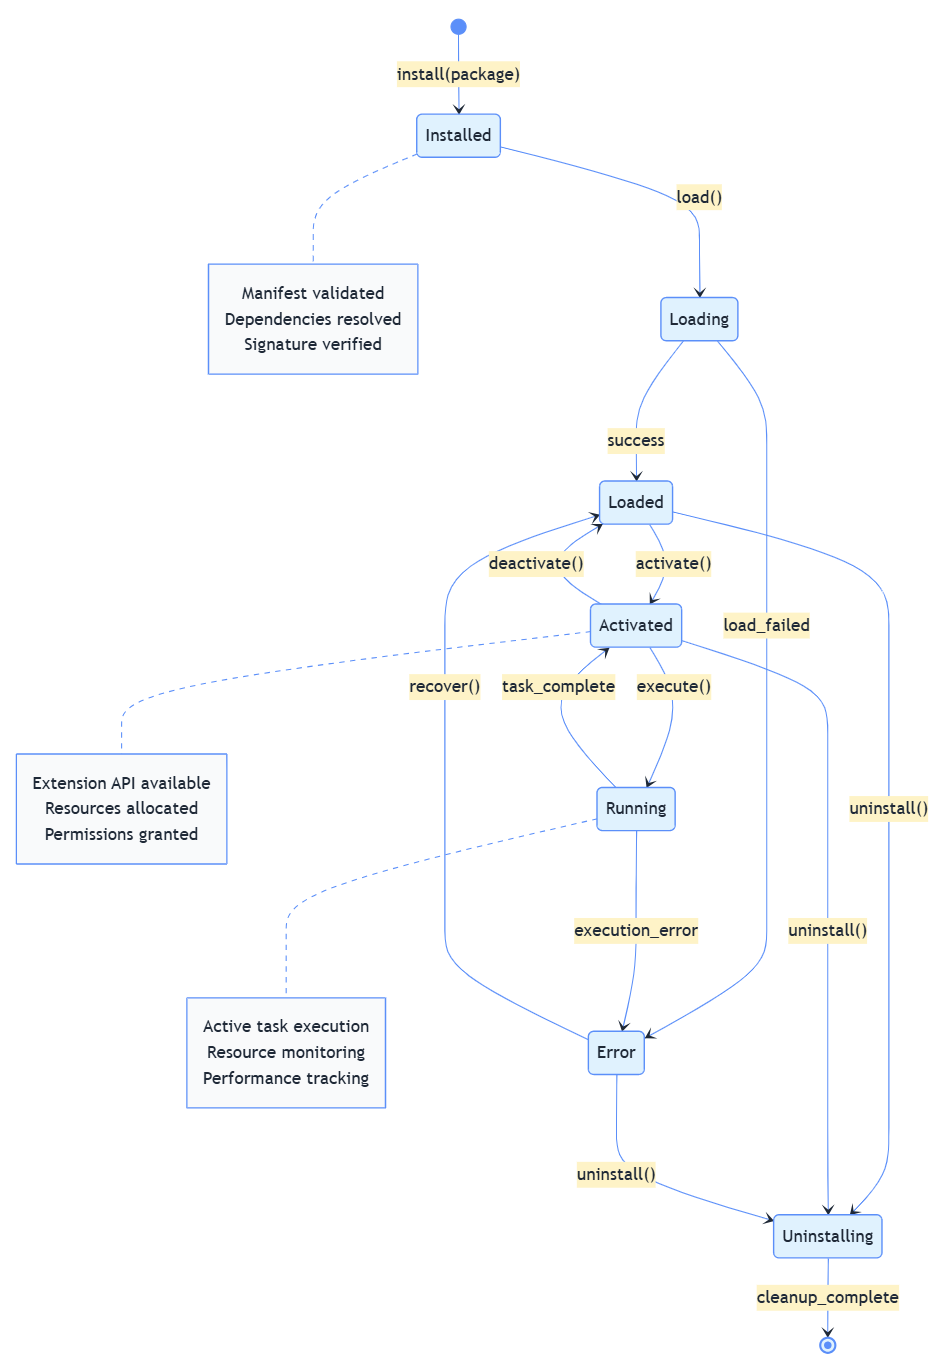
\includegraphics[width=1.05\textwidth]{images/diagrams/state_diagram/1_extension_lifecycle_chambering.png}
\caption{Extension Lifecycle State Machine}
\label{fig:3.15-extension-lifecycle}
\end{figure}

\subsection*{3.7.4 Extension Installation State Management}

The installation process manages eight distinct states ensuring reliable extension deployment with comprehensive security validation, dependency resolution, and automatic rollback capabilities:

\begin{compactlist}
    \item \textbf{Browsing}: User selection validation in marketplace
    \item \textbf{Downloading}: Network connectivity and package integrity verification
    \item \textbf{Verifying}: Signature validation and malware scanning
    \item \textbf{ResolvingDeps}: Semantic versioning and conflict detection with automatic dependency download
    \item \textbf{Installing}: File system operations and registration
    \item \textbf{Installed}: Successfully deployed and ready for loading
    \item \textbf{RollingBack}: State restoration and cleanup for failed installations
    \item \textbf{Failed}: Detailed error logging and reporting
\end{compactlist}

This state machine addresses critical deployment challenges including security validation through comprehensive signature verification and integrity checks, dependency resolution with automatic detection and conflict resolution, rollback capability for failed installations with complete state restoration, and seamless user experience with detailed progress feedback and error reporting.

\subsection*{3.7.5 Extension Development Workflow}

The extension development workflow provides comprehensive tooling support through the Carets command-line interface. The workflow encompasses the complete development lifecycle from initial project creation through marketplace publication. Developers begin by scaffolding new extension projects with proper structure and manifests, then implement functionality using the provided SDK and APIs. The workflow includes integrated testing frameworks for validation, security signing for package integrity, and automated publication to the marketplace.

The development process emphasizes several key aspects. Automated scaffolding generates complete project structures with proper manifests and configuration files. Integrated testing provides comprehensive frameworks that validate functionality before publication. Security validation through cryptographic signing and verification ensures package integrity and authenticity. Marketplace integration enables seamless publication with automated quality checks and version management. The complete workflow guides developers through each stage systematically as illustrated in ~\ref{fig:3.16-extension-development}.

\begin{figure}[H]
\centering
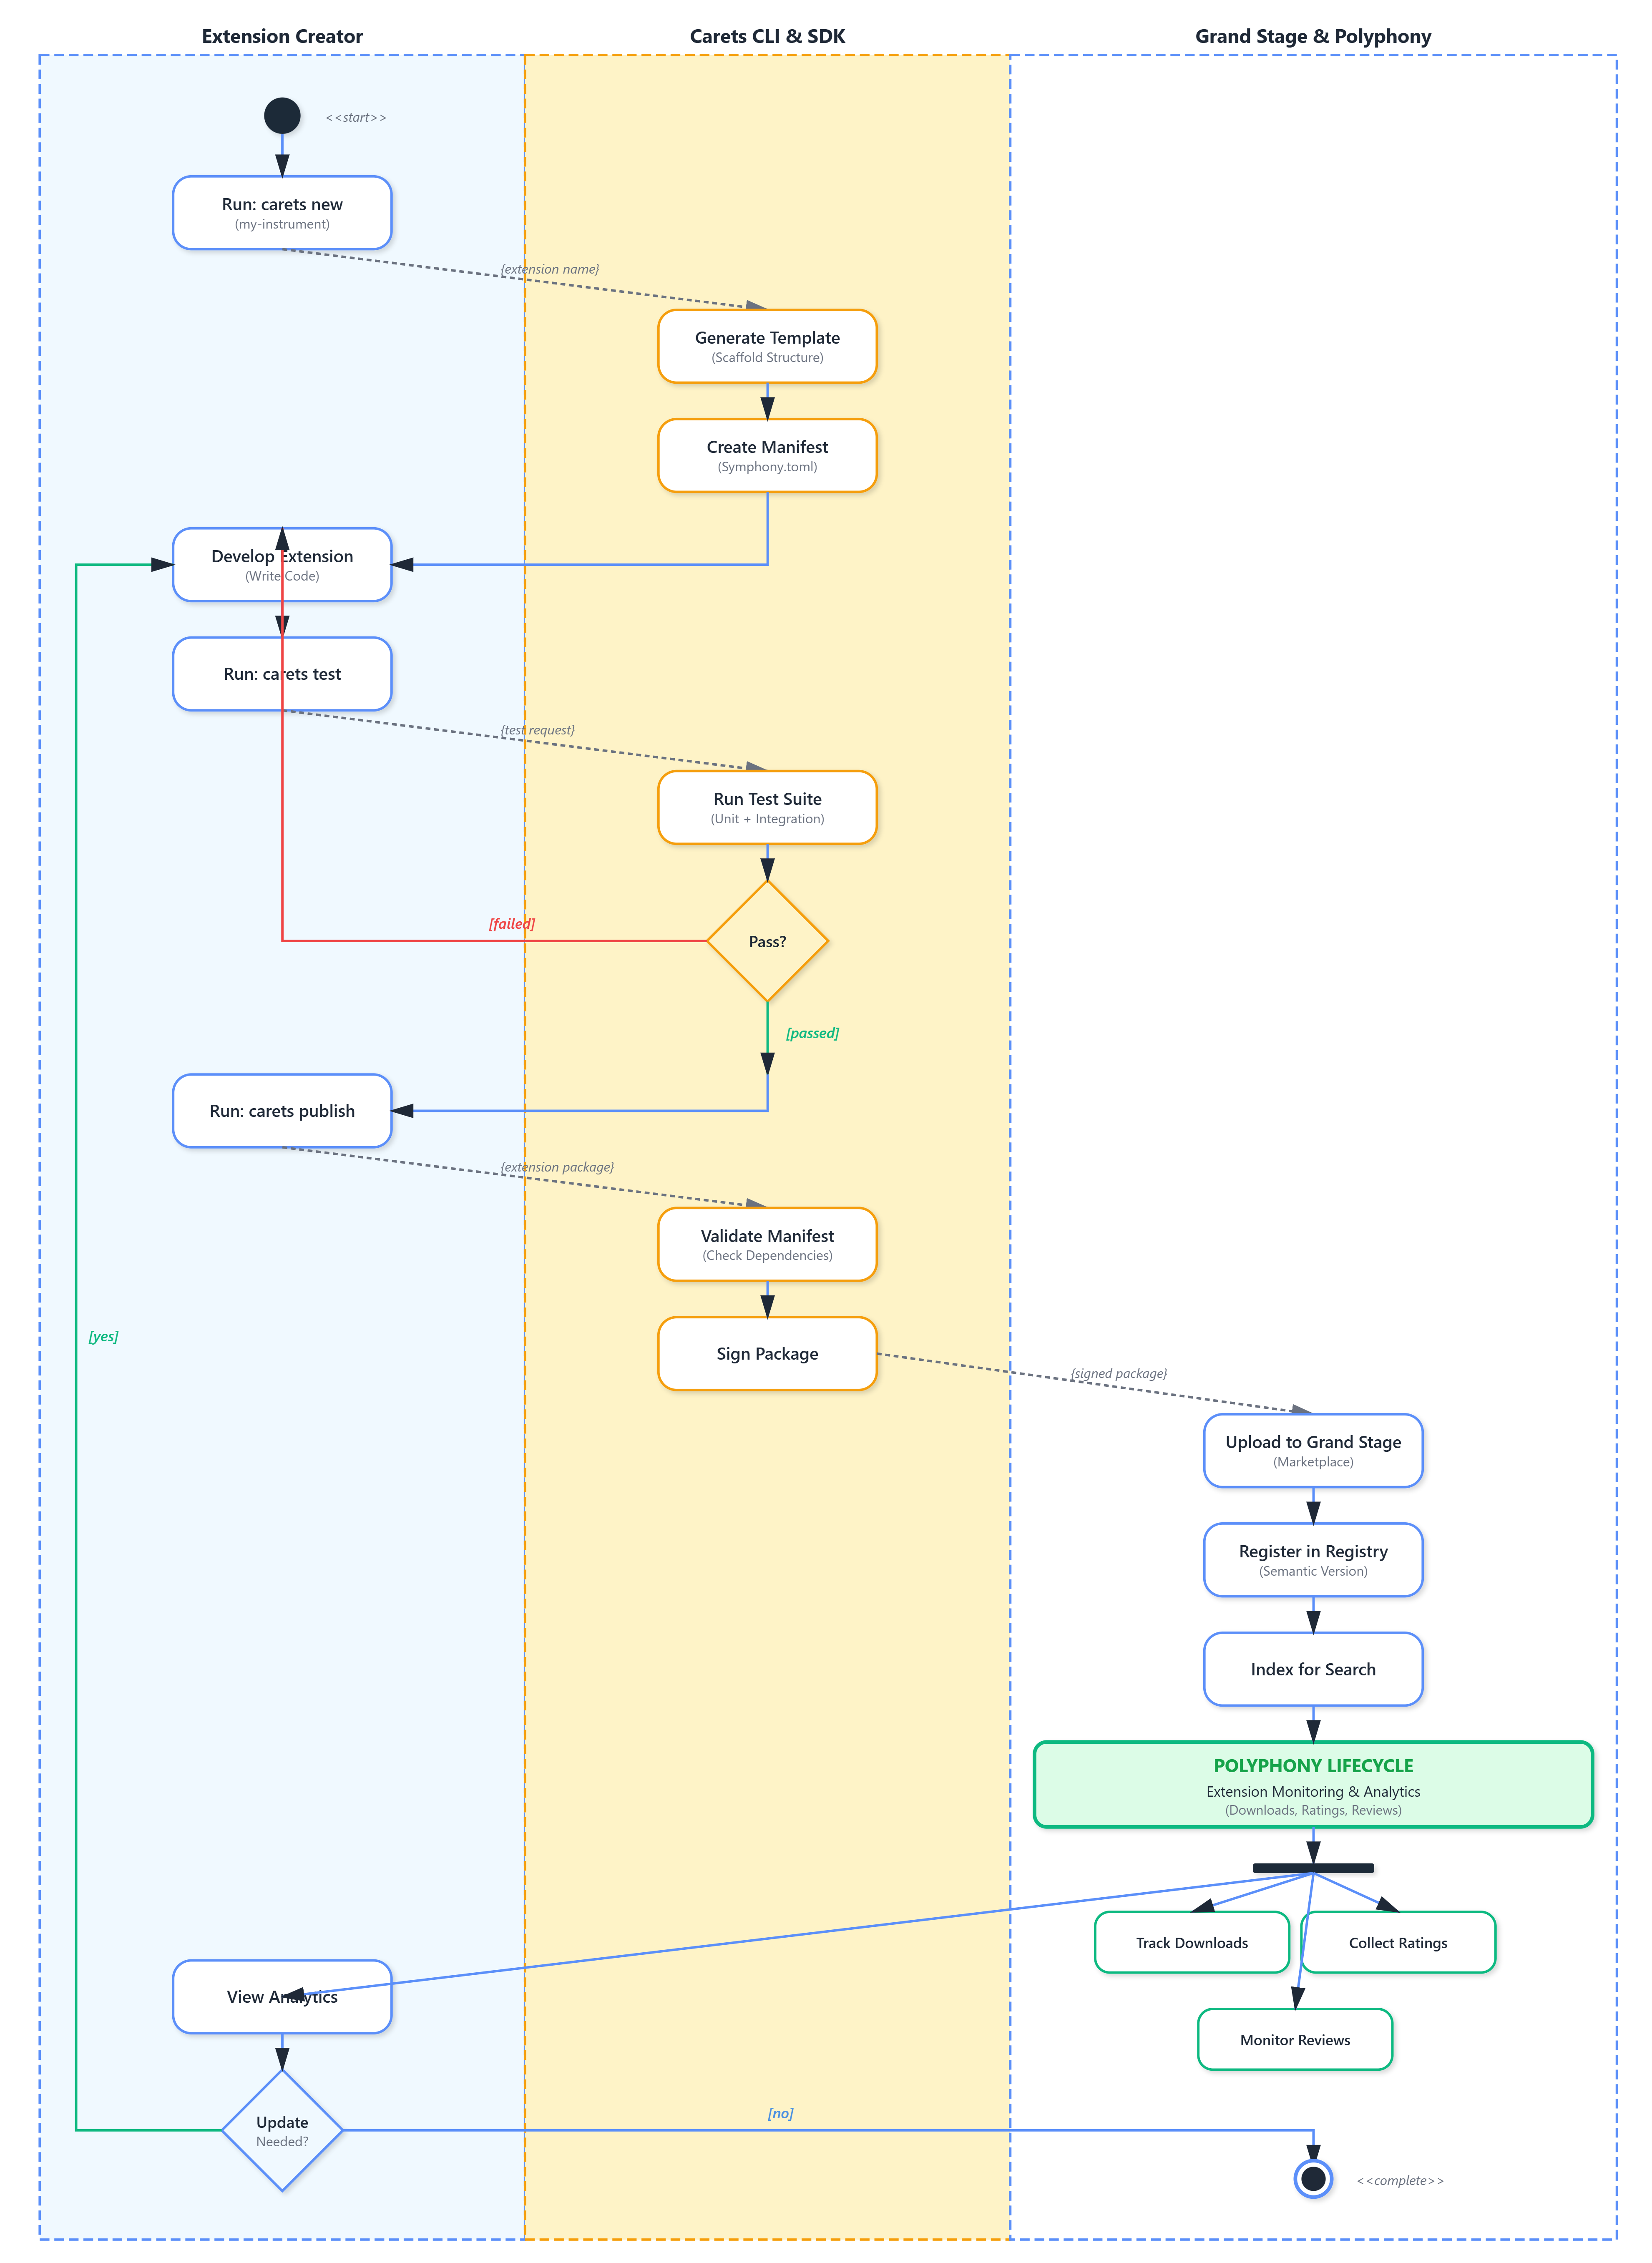
\includegraphics[width=1.15\textwidth]{images/diagrams/activity_diagram/symphony-extension-development.png}
\caption{Extension Development Workflow}
\label{fig:3.16-extension-development}
\end{figure}


% \subsection*{Marketplace and Ecosystem}

% The Grand Stage marketplace serves as the primary distribution channel for community and commercial extensions, implementing discovery through intelligent categorization and search capabilities, trust through comprehensive review processes and security scanning, quality through performance monitoring and user feedback, and sustainability through multiple monetization models supporting extension creator businesses.

% The marketplace supports multiple monetization strategies creating a sustainable ecosystem:

% \begin{compactlist}
%     \item \textbf{Free and Open Source}: Community-driven development and reputation building
%     \item \textbf{Freemium}: Basic functionality free with premium features available
%     \item \textbf{Usage-Based}: Pricing tied to actual consumption of resources or API calls
%     \item \textbf{Subscription}: Regular access fees for ongoing value delivery
%     \item \textbf{Enterprise Licensing}: Custom arrangements for organizational deployments
% \end{compactlist}

% Organizations can extend the public marketplace with private extension capabilities including internal-only extensions for proprietary workflows, role-based permissions for extension installation and usage, audit trails and governance controls for regulated environments, and professional services for specialized extension creation.


% Section 3.5: Orchestration System Design
% Section 3.8: Orchestration System Design
\clearpage
\section{3.8 Orchestration System Design}
\label{sec:orchestration-system}
\addcontentsline{toc}{section}{3.8 Orchestration System Design}

\lettrine{T}{his section} explores Symphony's orchestration system, the intelligence layer that coordinates multiple AI agents and tools to accomplish complex development tasks. We examine the Conductor's reinforcement learning approach, the Melody workflow abstraction, and the execution mechanisms that enable Agent-Driven Development. The orchestration system transforms high-level developer intent into concrete, executable workflows while continuously learning and improving from experience.

\subsection*{3.8.1 The Conductor and Reinforcement Learning}
\addcontentsline{toc}{subsection}{3.8.1 The Conductor and Reinforcement Learning}

The orchestration system represents the intelligence layer that enables Symphony to coordinate multiple AI agents and tools to accomplish complex development tasks. The orchestration philosophy embraces Agent-Driven Development, where specialized AI agents collaborate under intelligent coordination to handle implementation details while developers provide vision and strategic guidance.

The Conductor serves as the central intelligence within the orchestration system, implementing a reinforcement learning model that learns optimal workflow patterns from experience. The Conductor analyzes developer prompts to understand intent, examines project context, selects appropriate extensions and models for each task, determines execution sequence, and monitors execution for optimization opportunities. This intelligent coordination enables automatic workflow generation, significantly reducing cognitive load.

The system architecture consists of two main components that work together seamlessly:

\clearpage
\textbf{Component 1: IPC Communication Infrastructure}

The Conductor communicates with the core system through an inter-process communication infrastructure enabling seamless integration despite being implemented in Python while the core is in Rust. The IpcBus provides reliable message passing with Transport layer supporting Unix sockets (Linux/macOS) and named pipes (Windows). The Protocol layer handles message serialization and deserialization, ensuring safe data transmission between processes. The Security layer implements authentication and rate limiting to protect against malicious extensions. The Message component carries data with unique IDs, sender/receiver process IDs, payload bytes, and timestamps as illustrated in ~\ref{fig:3.17-ipc-infrastructure}.

\begin{figure}[H]
\centering
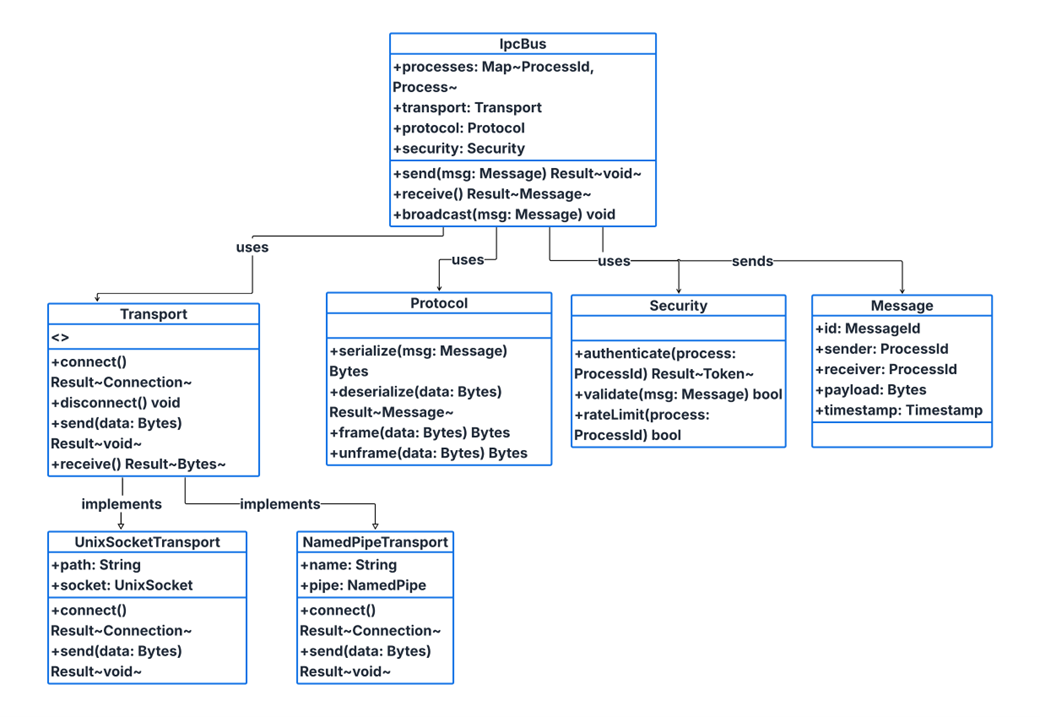
\includegraphics[width=1.20\textwidth]{images/diagrams/class_diagram/seperate_3_ipc_communication_conductor_rl/IPC Communication Infrastructure.png}
\caption{IPC Communication Infrastructure}
\label{fig:3.17-ipc-infrastructure}
\end{figure}

\clearpage
\textbf{Component 2: Conductor Architecture}

The Conductor component integrates the reinforcement learning model with the orchestration system. The RlModel implements the policy and value function, predicting actions from states and updating through experience. The OrchestrationBridge converts between Melody workflows and DAG structures, collecting execution rewards. The PyO3Bindings enable seamless Rust-Python interoperability, converting values between languages and calling Python functions from Rust. This architecture enables the Conductor to leverage Python's ML ecosystem while maintaining Rust core performance as illustrated in ~\ref{fig:3.18-conductor-architecture}.

\begin{figure}[H]
\centering
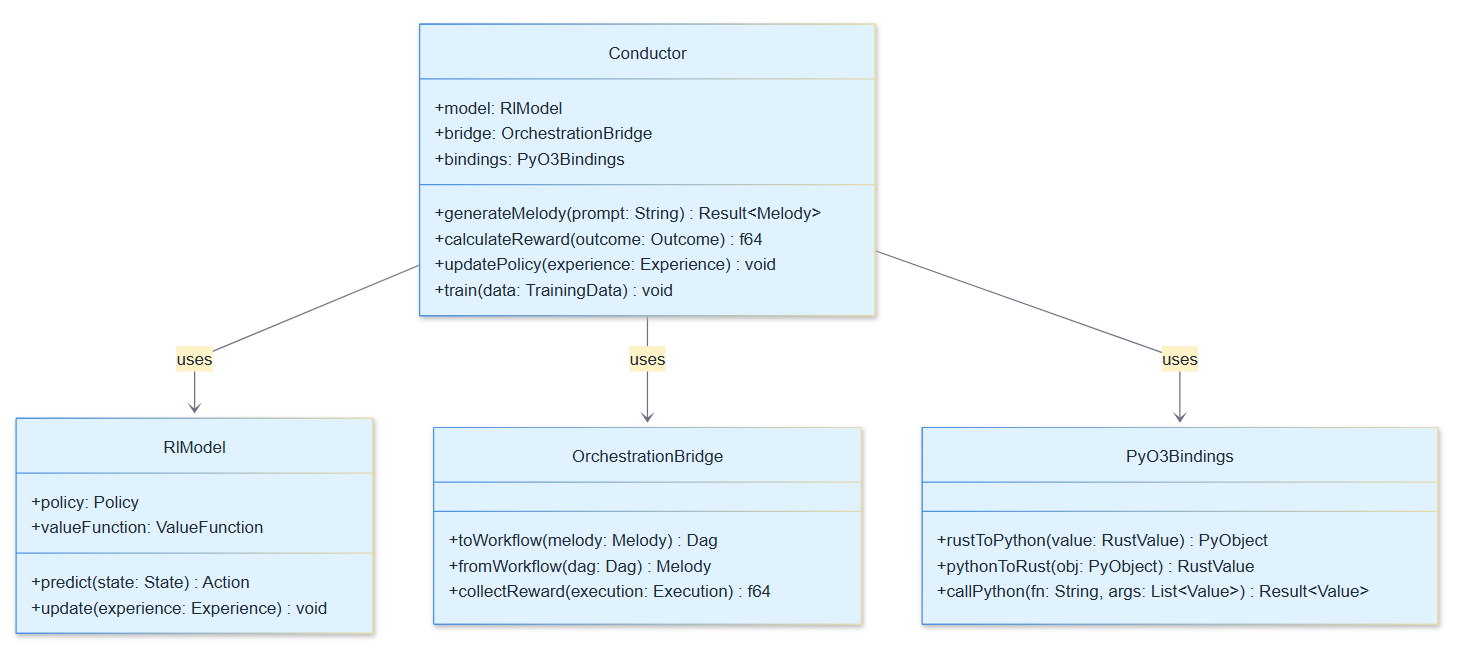
\includegraphics[width=1.20\textwidth]{images/diagrams/class_diagram/seperate_3_ipc_communication_conductor_rl/Conductor Architecture.png}
\caption{Conductor Architecture - RL Model and Integration Components}
\label{fig:3.18-conductor-architecture}
\end{figure}

\clearpage
The reinforcement learning model learns from every workflow execution, continuously improving its ability to generate effective task sequences. The model treats workflow generation as a sequential decision problem, selecting the next task based on current state. The state representation includes developer prompt, project context, existing workflow tasks, and available extensions. The model outputs a probability distribution over possible next tasks, sampling to generate diverse workflows.

The reward signal drives learning from multiple sources: execution success (objective accomplishment), execution time (efficiency), artifact quality (output value), and user feedback (developer satisfaction). These components combine into a single scalar value guiding the learning process. The model updates parameters after each execution using policy gradient methods, increasing probability of high-reward actions and decreasing probability of low-reward actions.


% \clearpage
\subsection*{3.8.2 Melody System and Workflow Generation}
\addcontentsline{toc}{subsection}{3.8.2 Melody System and Workflow Generation}

The Melody concept provides the abstraction through which developers interact with workflows in Symphony. A Melody represents a complete workflow as a directed acyclic graph where nodes represent individual tasks and edges represent dependencies between tasks. Melodies can be created manually through the visual Harmony Board interface or generated automatically by the Conductor based on natural language prompts. Once created, Melodies can be saved, shared, and reused, building up a library of proven workflows for common development tasks. The Melody abstraction enables developers to think about workflows at a high level without concerning themselves with the details of how individual tasks are implemented or coordinated.

The execution of a Melody involves multiple system components working together in a coordinated fashion, which can be understood through three distinct phases:

\clearpage
\textbf{Phase 1: Orchestration Flow}

The workflow begins when the developer writes a prompt describing the desired outcome. The Frontend UI submits this prompt to the Core system, which forwards it to the Conductor for processing. The Conductor analyzes the prompt and generates a Melody workflow. In Maestro Mode, the Conductor uses reinforcement learning to automatically generate the workflow. In Manual Mode, the system requests the developer to select from available Melodies through a browser interface. Once the Melody is selected or generated, the Conductor orchestrates its execution as illustrated in ~\ref{fig:3.19-melody-orchestration}.

\begin{figure}[H]
\centering
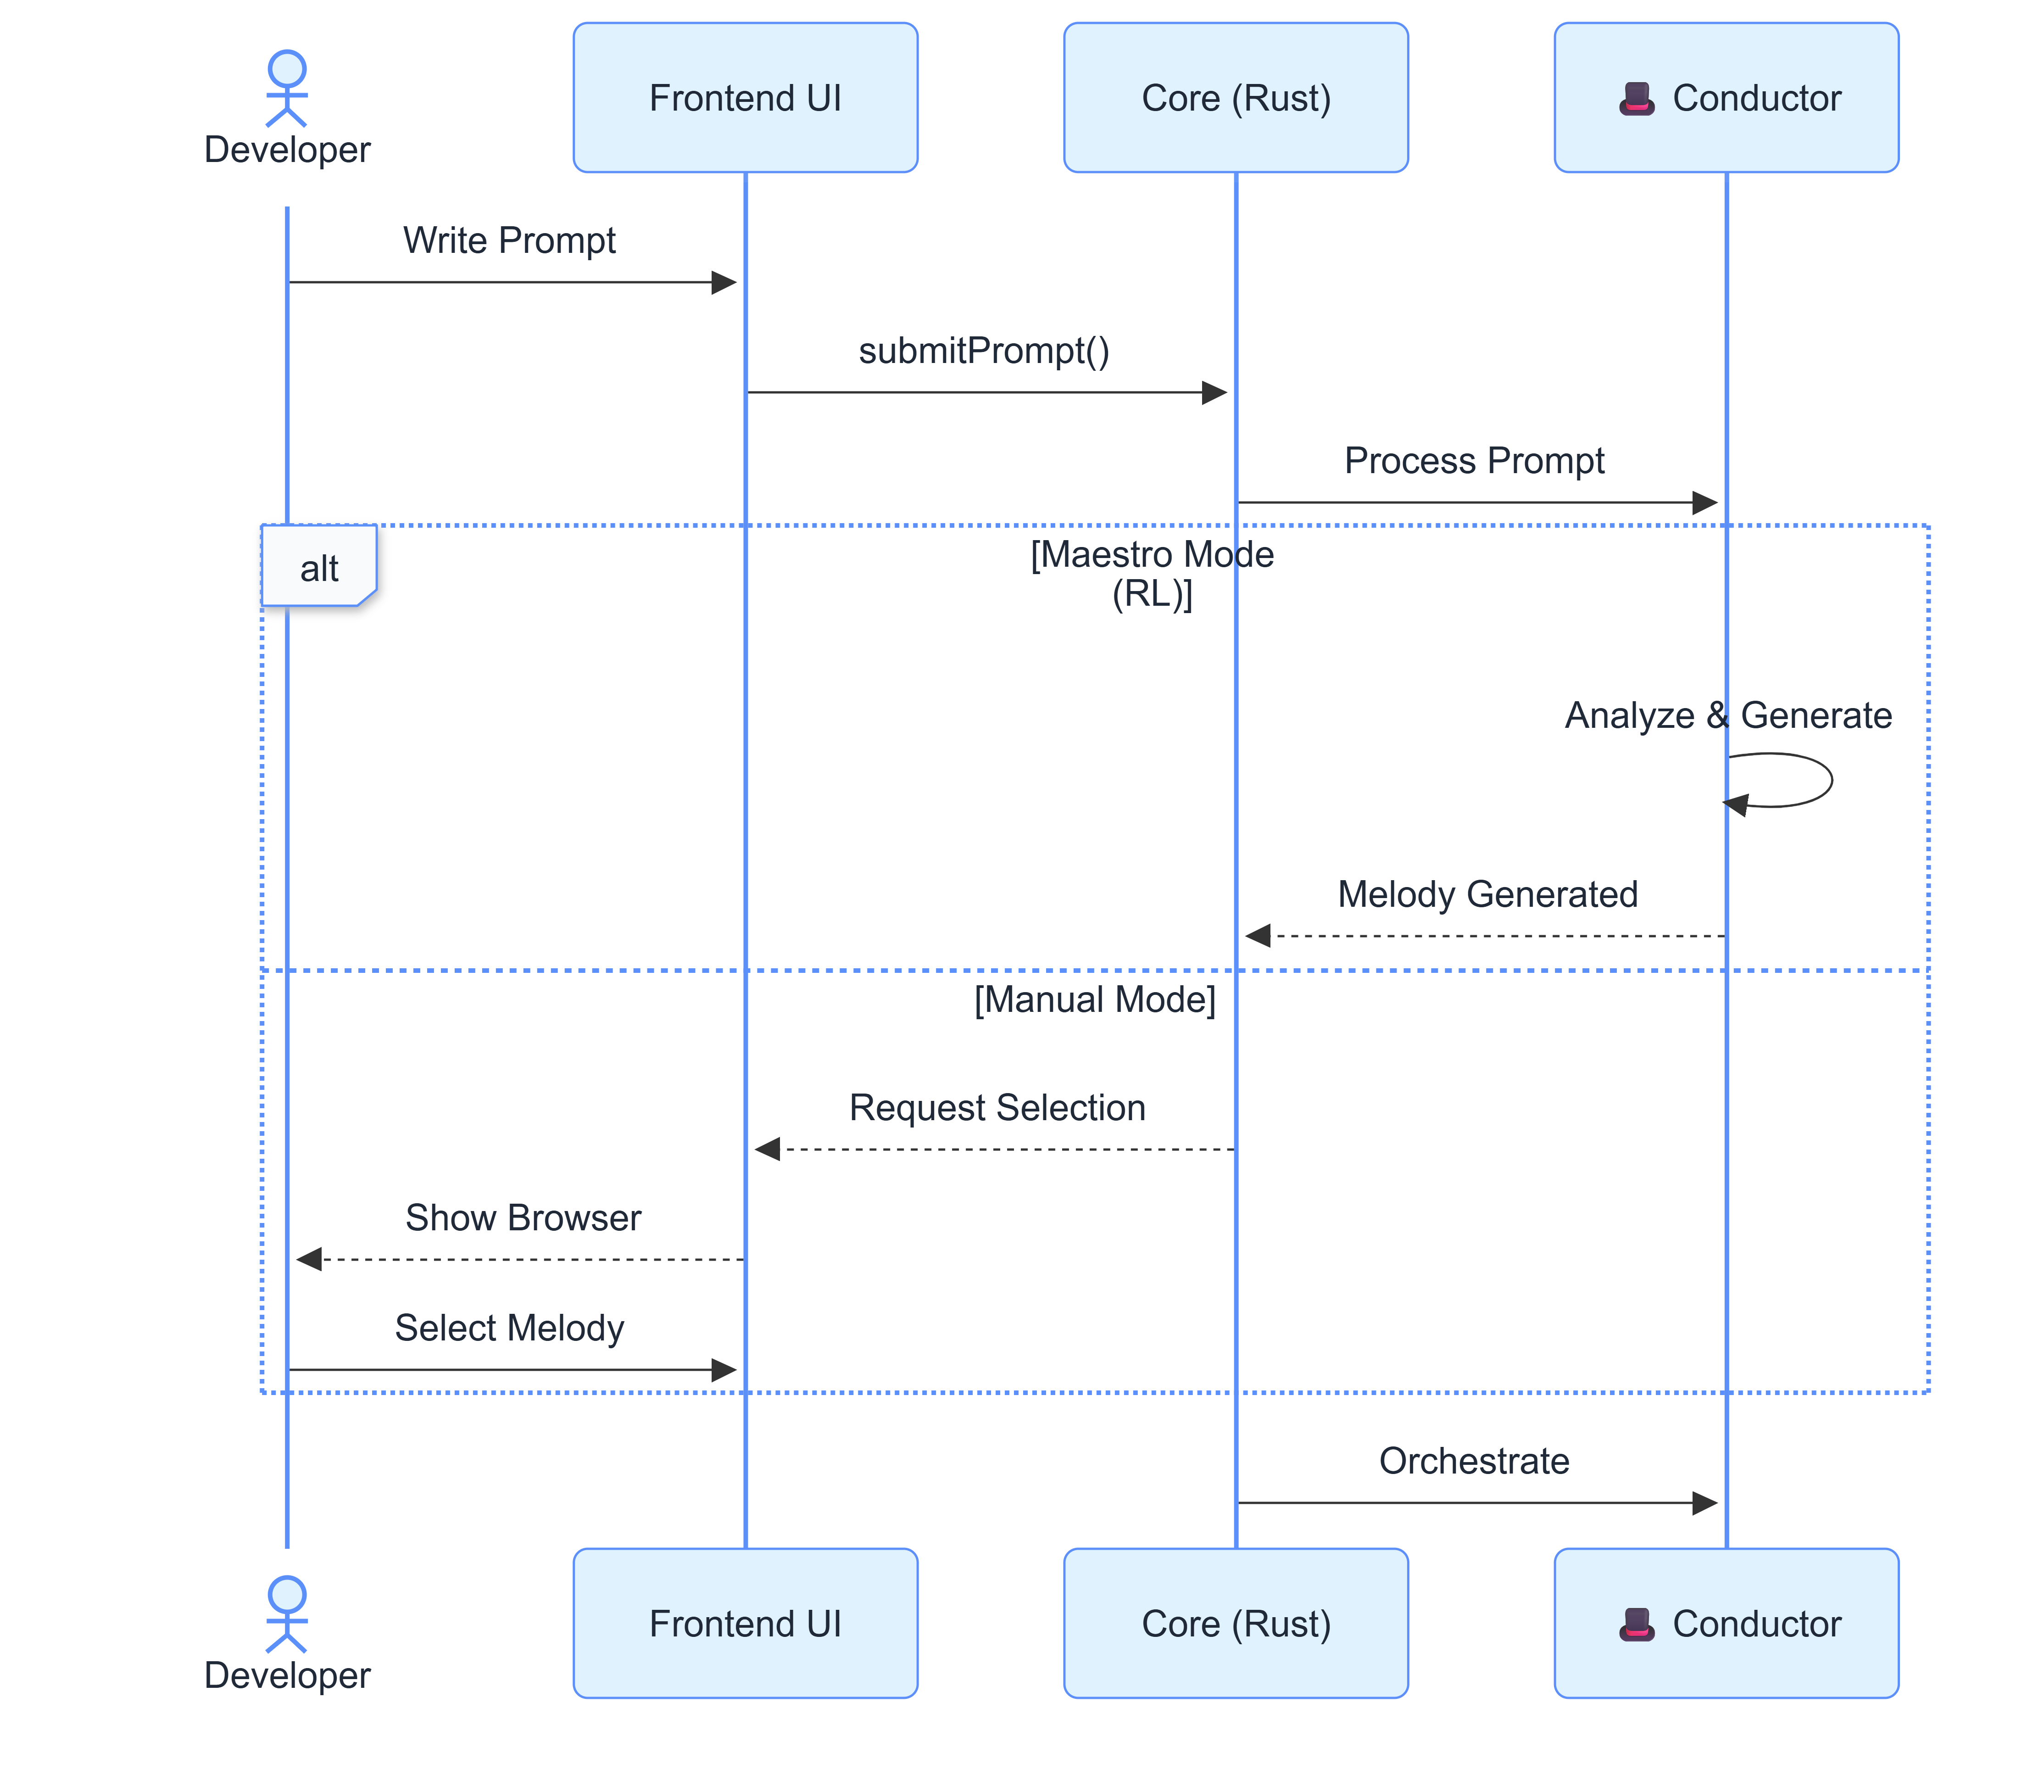
\includegraphics[width=0.95\textwidth]{images/diagrams/sequence_diagram/seperate_1_developer_workflow_execute_melody/Orchestration Flow.png}
\caption{Melody Orchestration Flow}
\label{fig:3.19-melody-orchestration}
\end{figure}

\clearpage
\textbf{Phase 2: Execution Flow}

After orchestration, the Conductor dispatches tasks to The Pit for execution. The Pit coordinates with the Pool Manager to allocate Player extensions, ensuring required AI models and tools are ready. The DAG Tracker manages task execution order based on dependencies, running each task in sequence or parallel as appropriate. As tasks complete, their results are stored in the ArtifactStore with unique identifiers. The Pit monitors execution progress and handles any errors that occur during task processing as illustrated in ~\ref{fig:3.20-melody-execution}.

\begin{figure}[H]
\centering
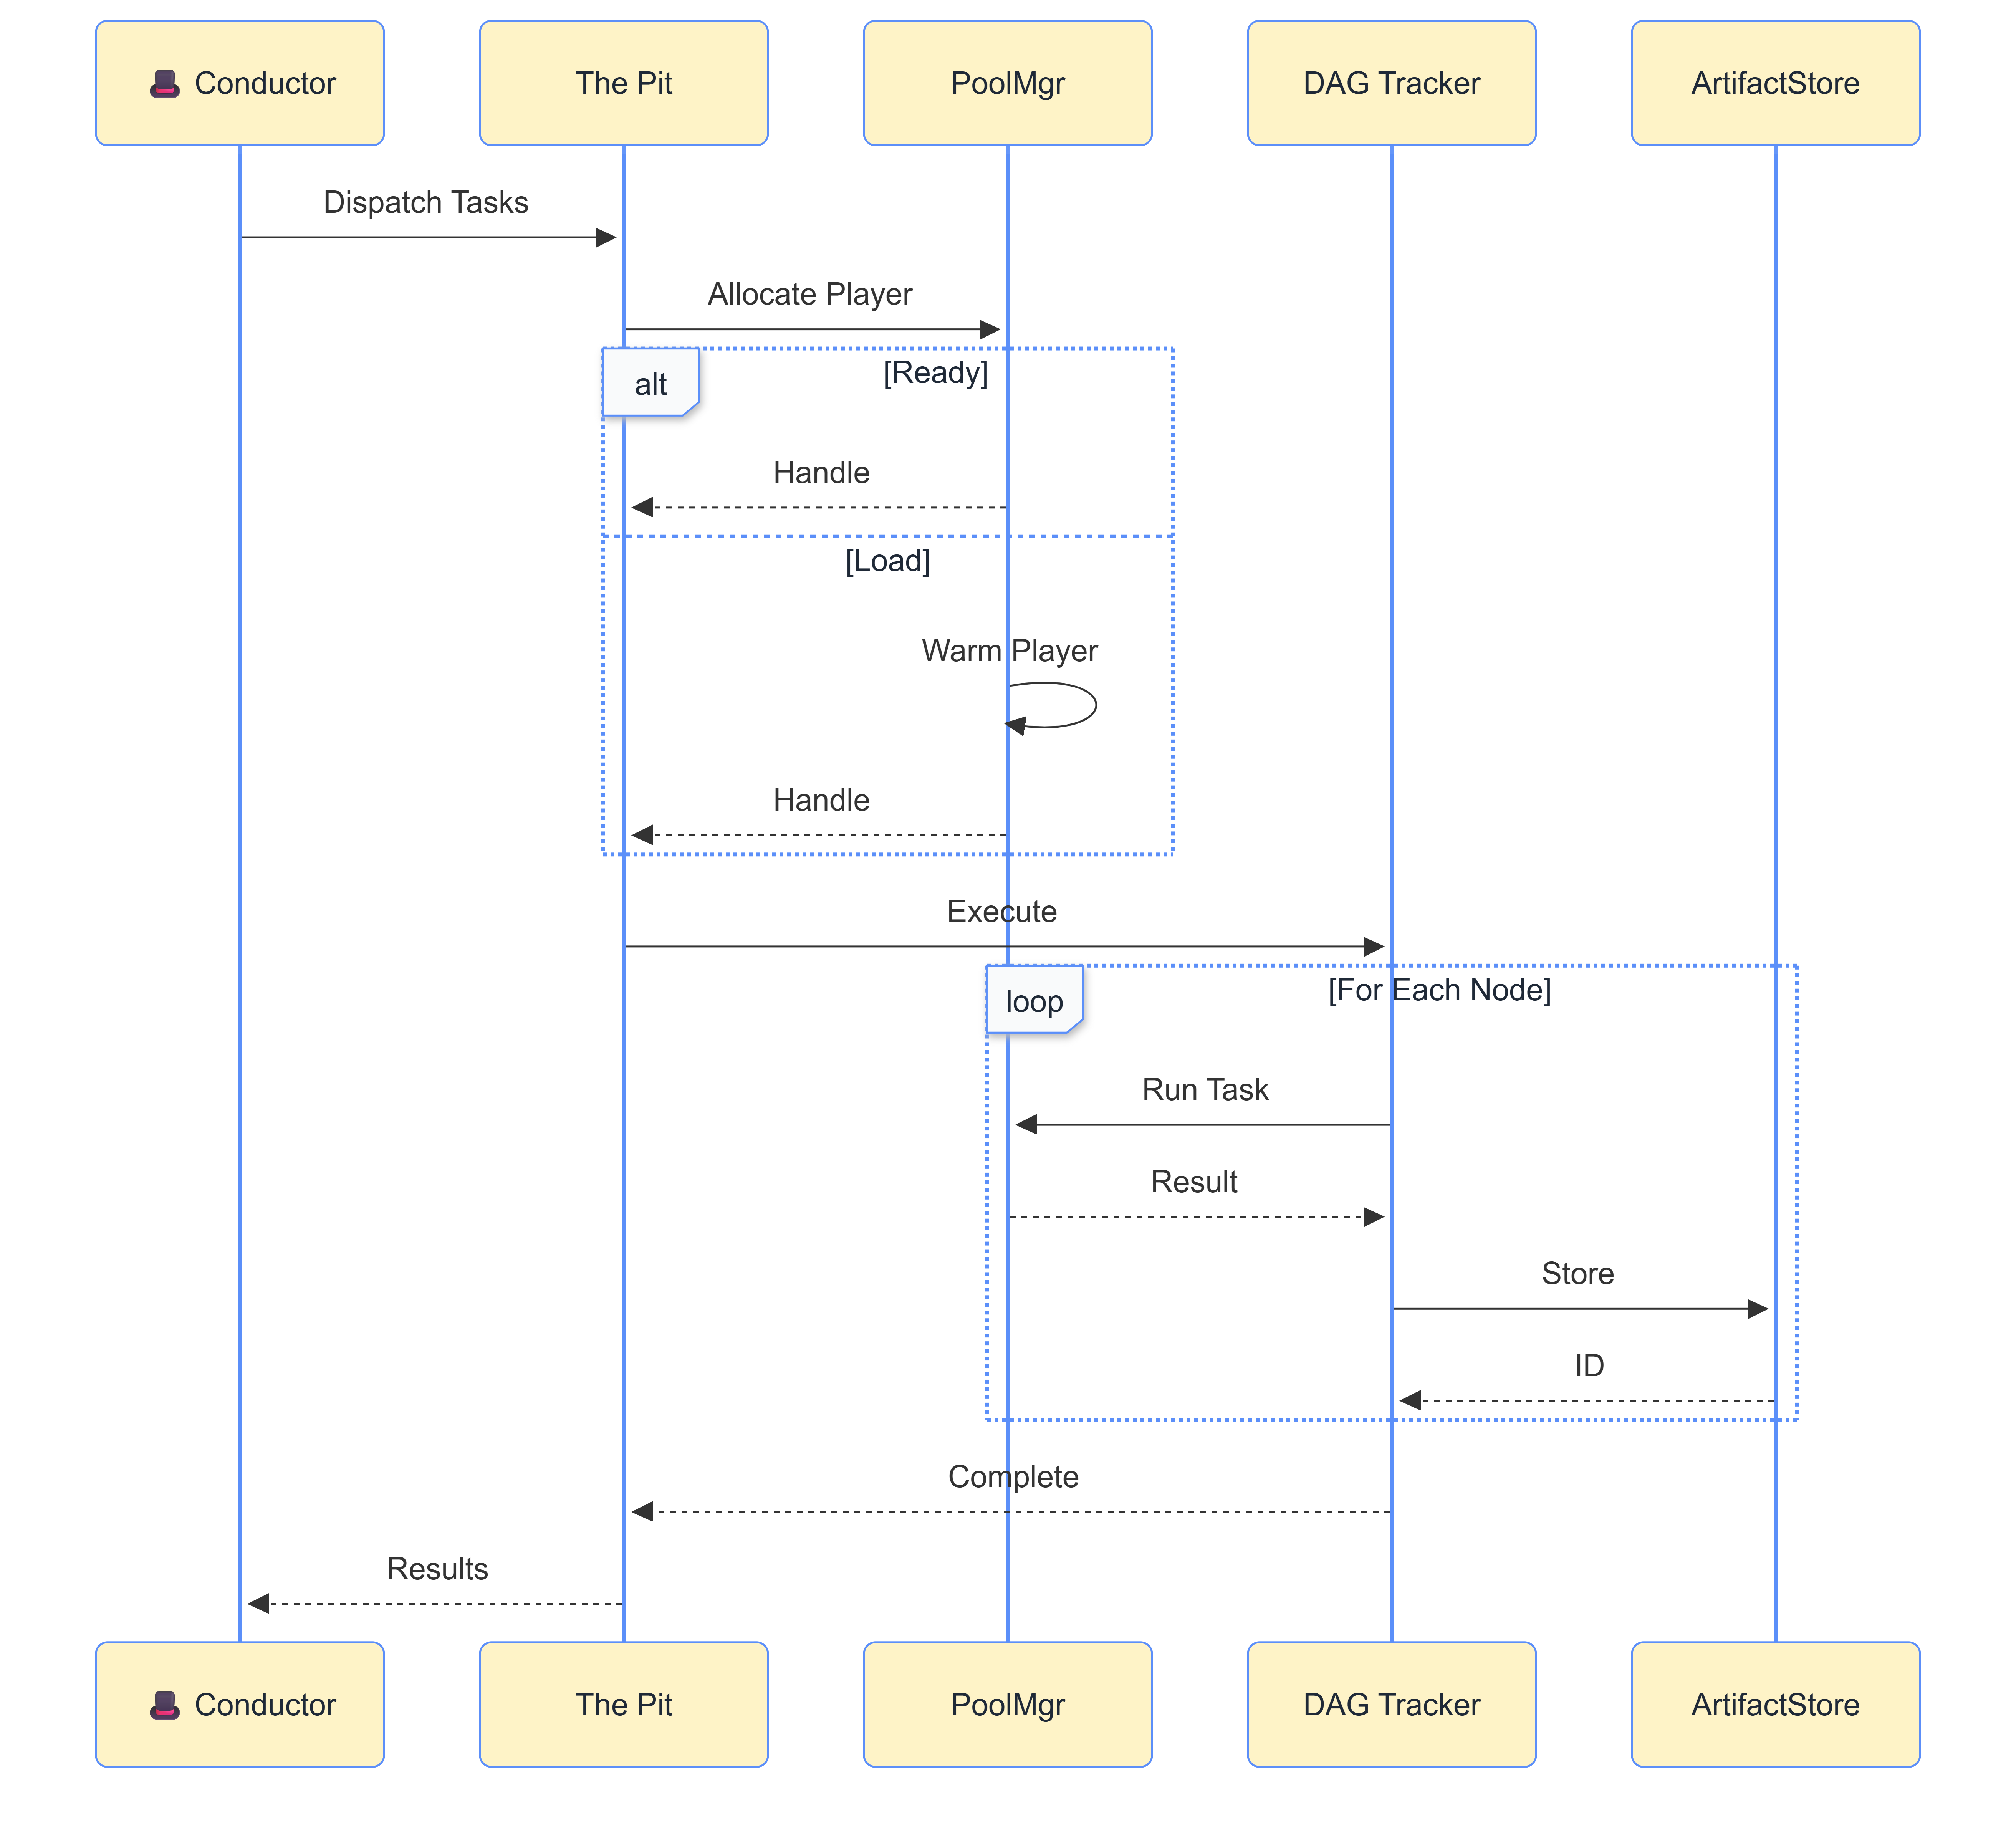
\includegraphics[width=0.95\textwidth]{images/diagrams/sequence_diagram/seperate_1_developer_workflow_execute_melody/Execution Flow.png}
\caption{Melody Execution Flow}
\label{fig:3.20-melody-execution}
\end{figure}

\clearpage
\textbf{Phase 3: Data Retrieval Flow}

Once execution completes, the Core system sends status updates to the Frontend UI, which displays results to the developer. When the developer requests to view artifacts, the UI queries the Core system, which retrieves data from the ArtifactStore. The stored artifacts are returned through the system layers and displayed to the developer. This completes the full Melody execution cycle, with the Conductor calculating rewards and updating its model to improve future workflow generation as illustrated in ~\ref{fig:3.21-melody-retrieval}.

\begin{figure}[H]
\centering
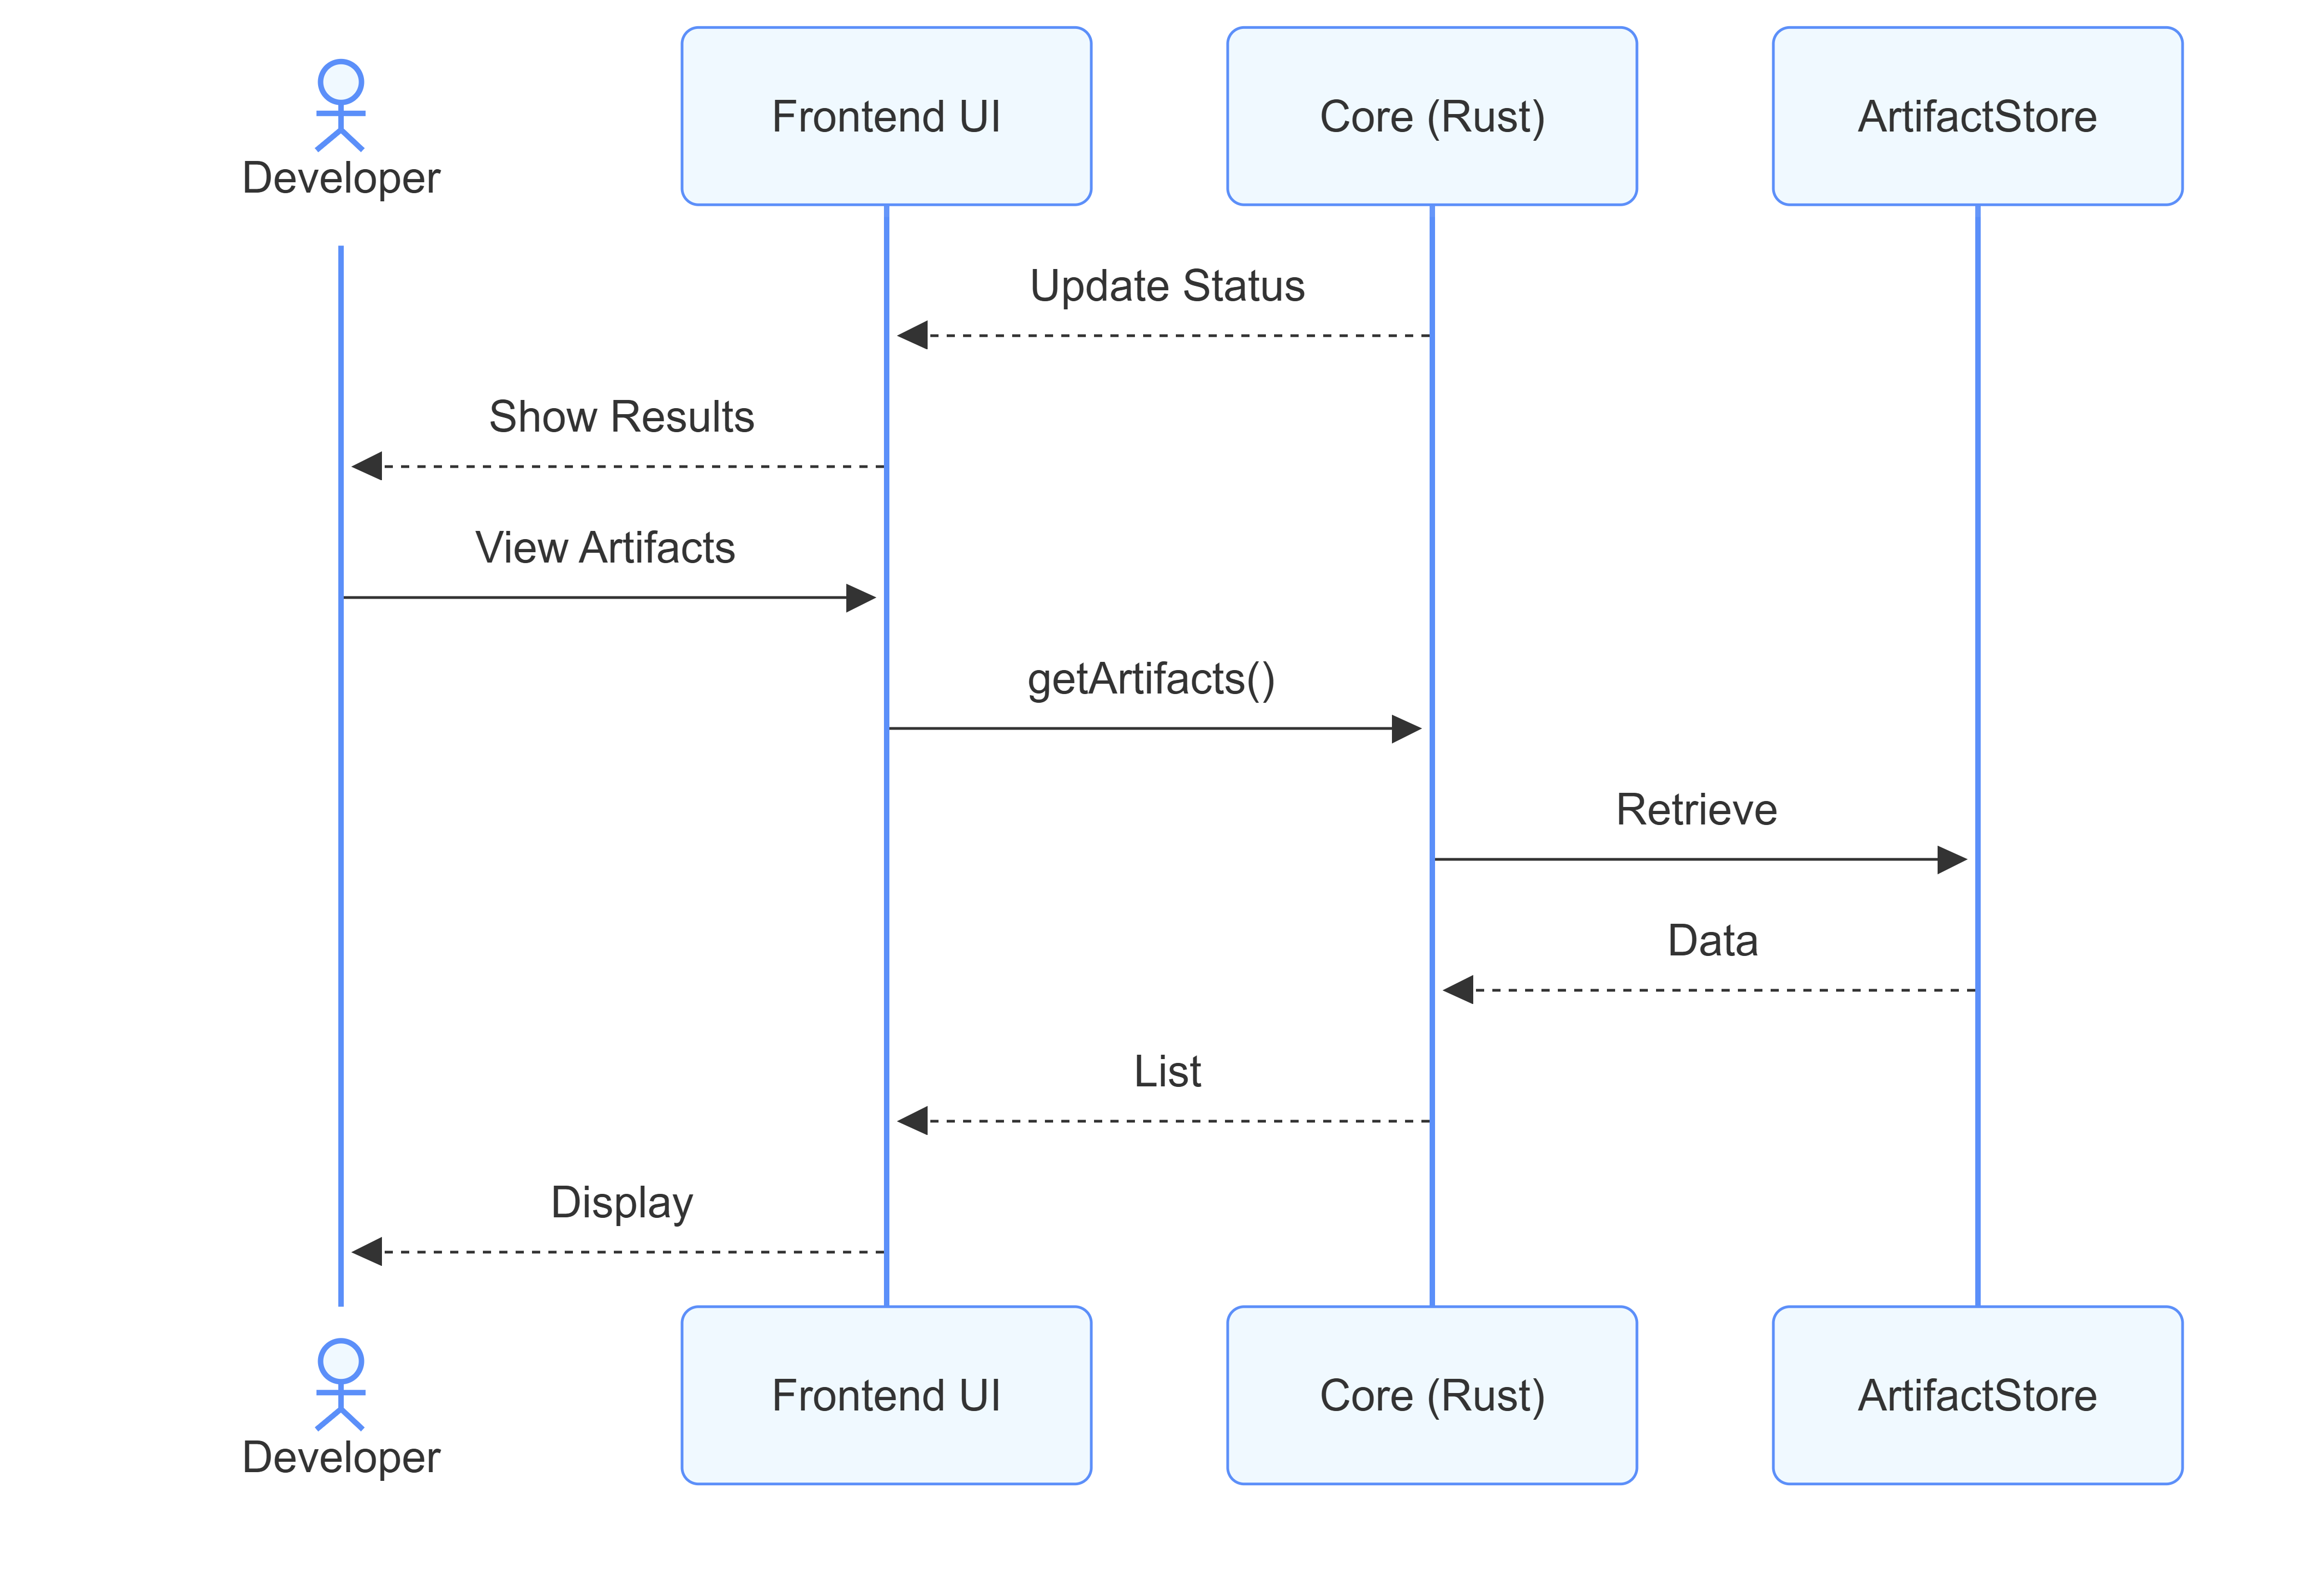
\includegraphics[width=0.95\textwidth]{images/diagrams/sequence_diagram/seperate_1_developer_workflow_execute_melody/Data Retrieval Flow.png}
\caption{Melody Data Retrieval Flow}
\label{fig:3.21-melody-retrieval}
\end{figure}

\clearpage

The workflow generation process implemented by the Conductor involves several sophisticated steps that transform a natural language prompt into an executable workflow, which can be understood through two main phases:

\textbf{Phase 1: Inference \& Generation}

The process begins with intent parsing, where the Conductor receives a complex prompt from the developer through the Frontend UI and Core system. The Conductor analyzes the prompt using natural language understanding techniques to extract key objectives, constraints, and preferences. It then queries the RL Model to get action probabilities through a forward pass. The RL Model generates an action distribution that guides workflow construction. The Conductor uses these probabilities to generate the workflow structure, with the Melody Engine creating a concrete workflow graph where nodes represent extension invocations and edges represent data dependencies. The generated Melody is then previewed to the developer through the UI, displaying the workflow graph for review before execution as illustrated in ~\ref{fig:3.22-conductor-inference}.

\begin{figure}[H]
\centering
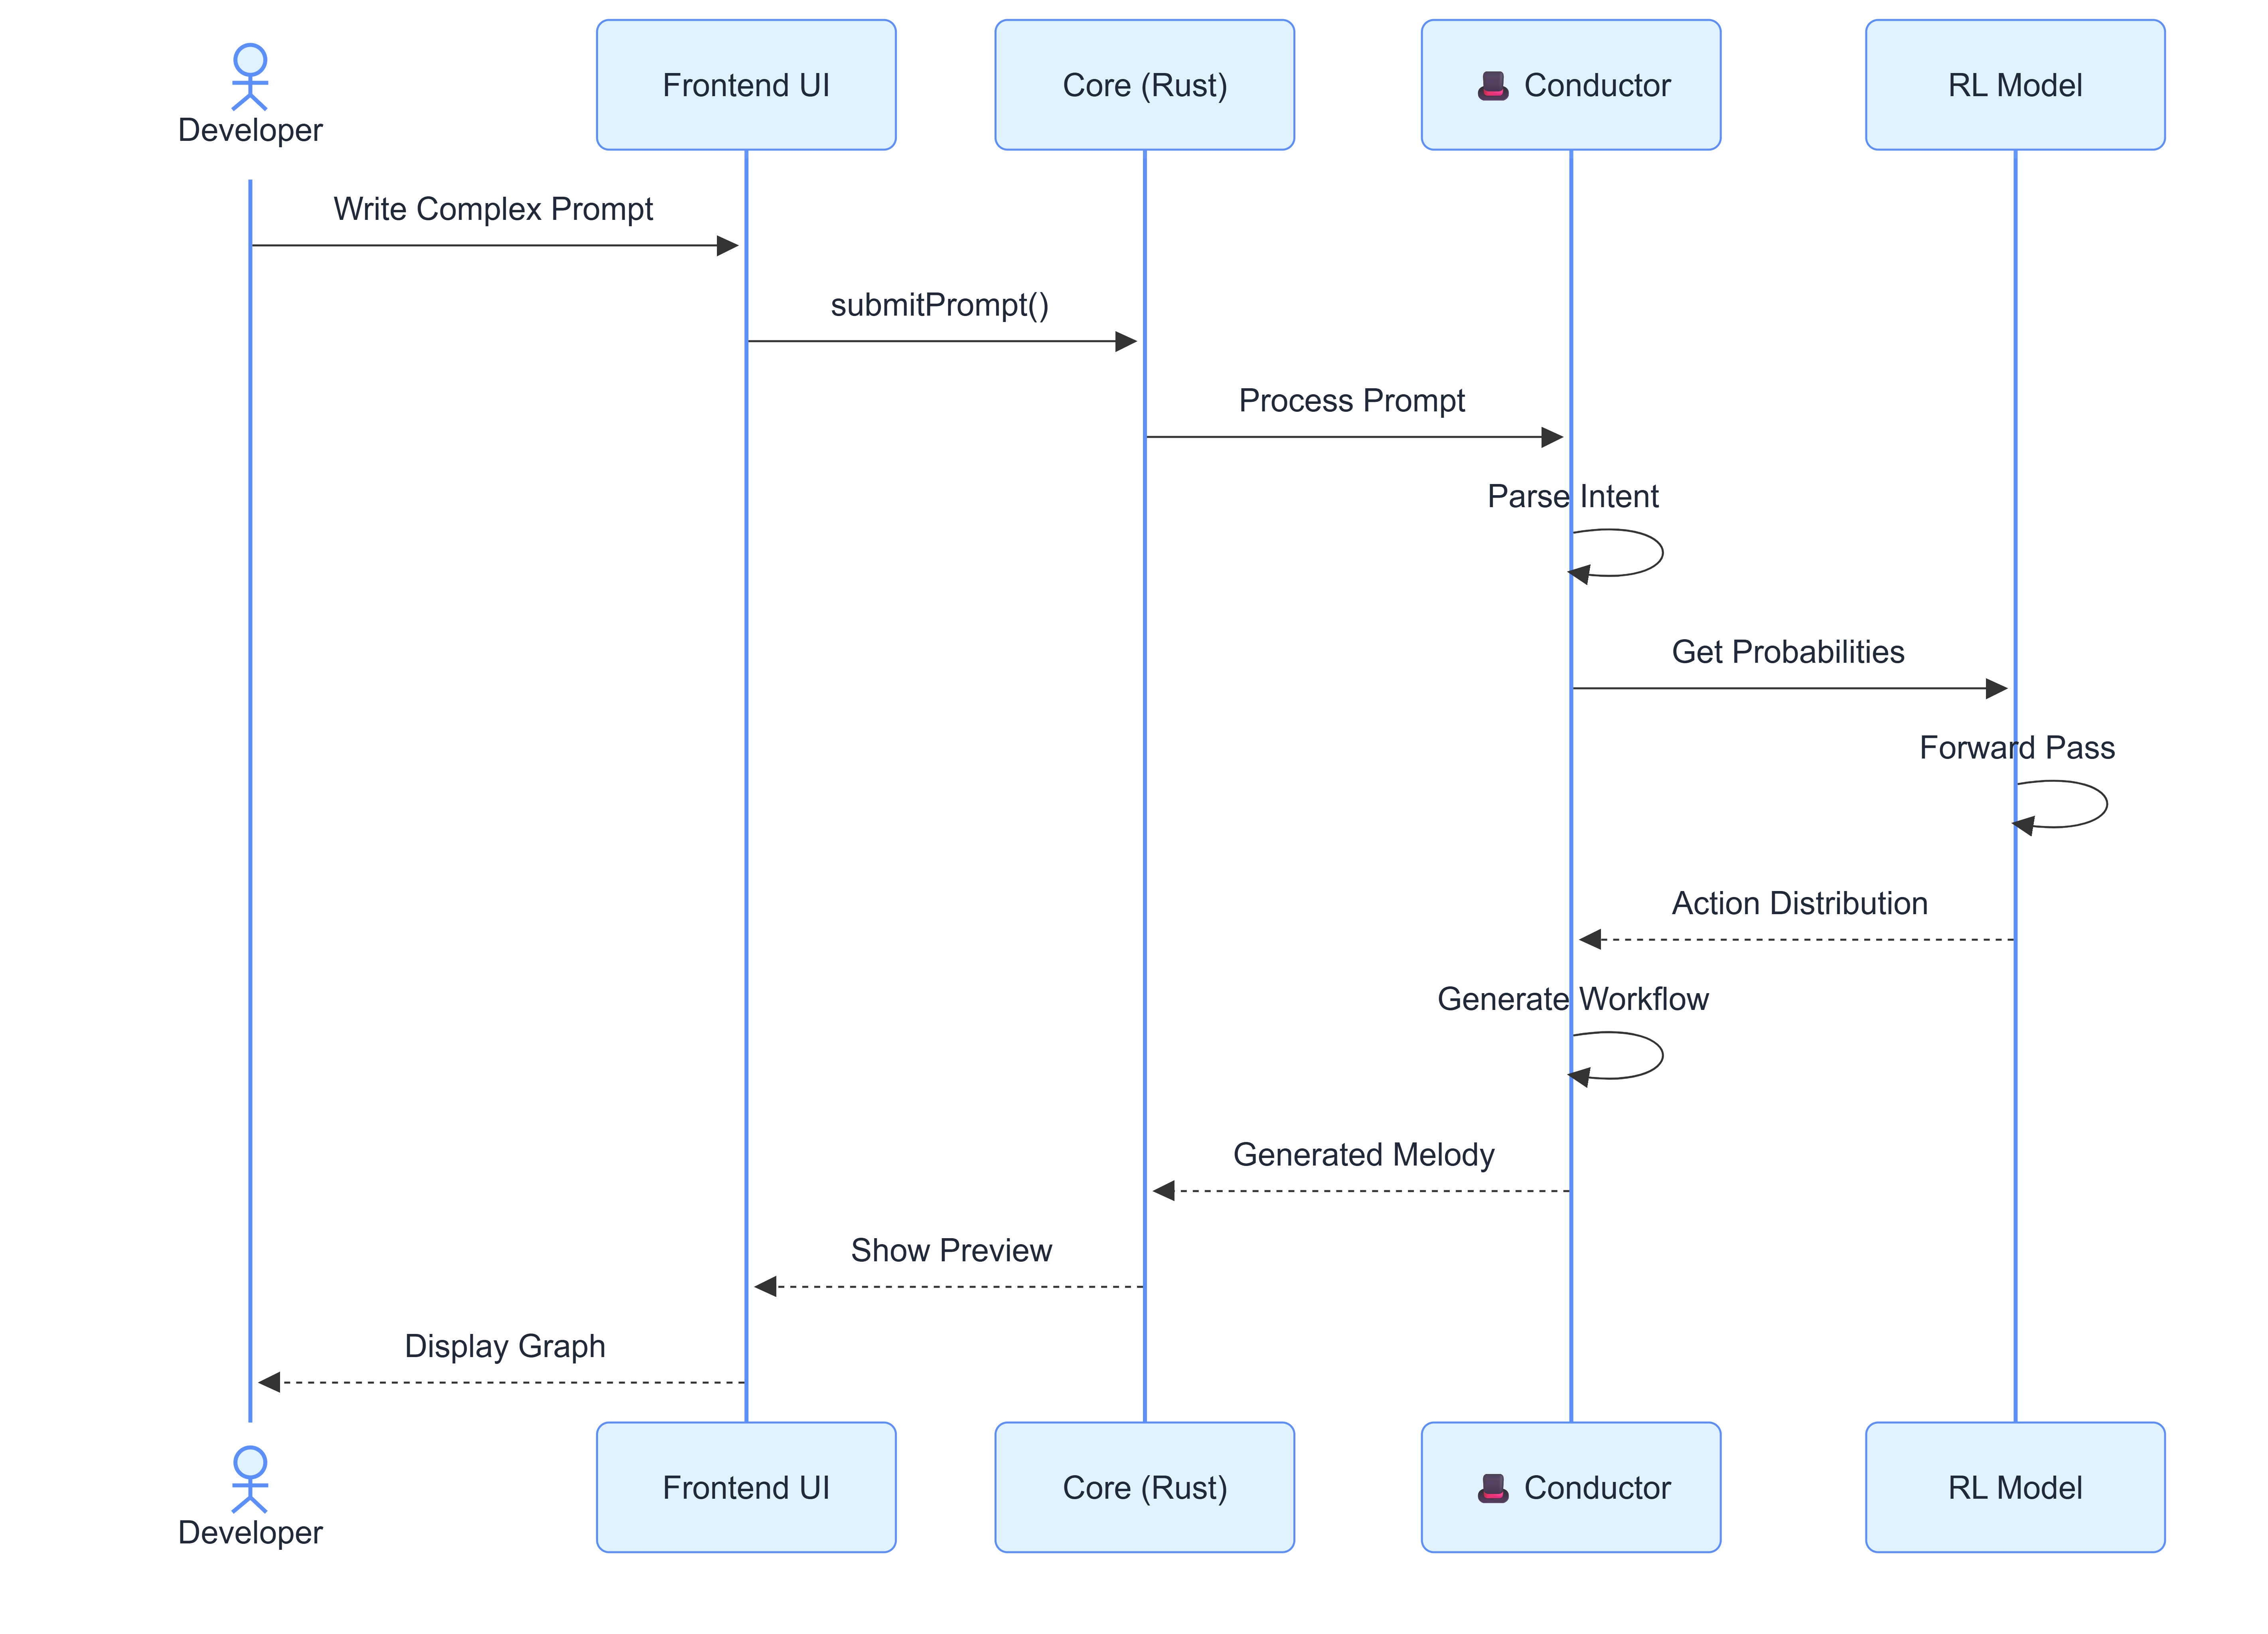
\includegraphics[width=0.95\textwidth]{images/diagrams/sequence_diagram/seperate_4_conductor_workflow_generate_melody/Inference & Generation.png}
\caption{Conductor Inference \& Generation Phase}
\label{fig:3.22-conductor-inference}
\end{figure}

\clearpage
\textbf{Phase 2: Execution \& Learning}

After the developer approves and executes the Melody, the Core system starts execution and the Conductor dispatches tasks to the Bridge component. During execution, the Conductor collects execution metrics including success rates, execution time, and artifact quality. These metrics are used to update the RL Model through backpropagation, implementing the reinforcement learning cycle where the model learns from experience. The RL Model calculates rewards based on the execution outcome (State → Action → Reward) and updates its parameters to improve future workflow generation. Optionally, the developer can save the successful Melody to the Polyphony marketplace, making it available for reuse by other developers. This continuous learning cycle enables the Conductor to improve its workflow generation capabilities over time as illustrated in ~\ref{fig:3.23-conductor-learning}.

\begin{figure}[H]
\centering
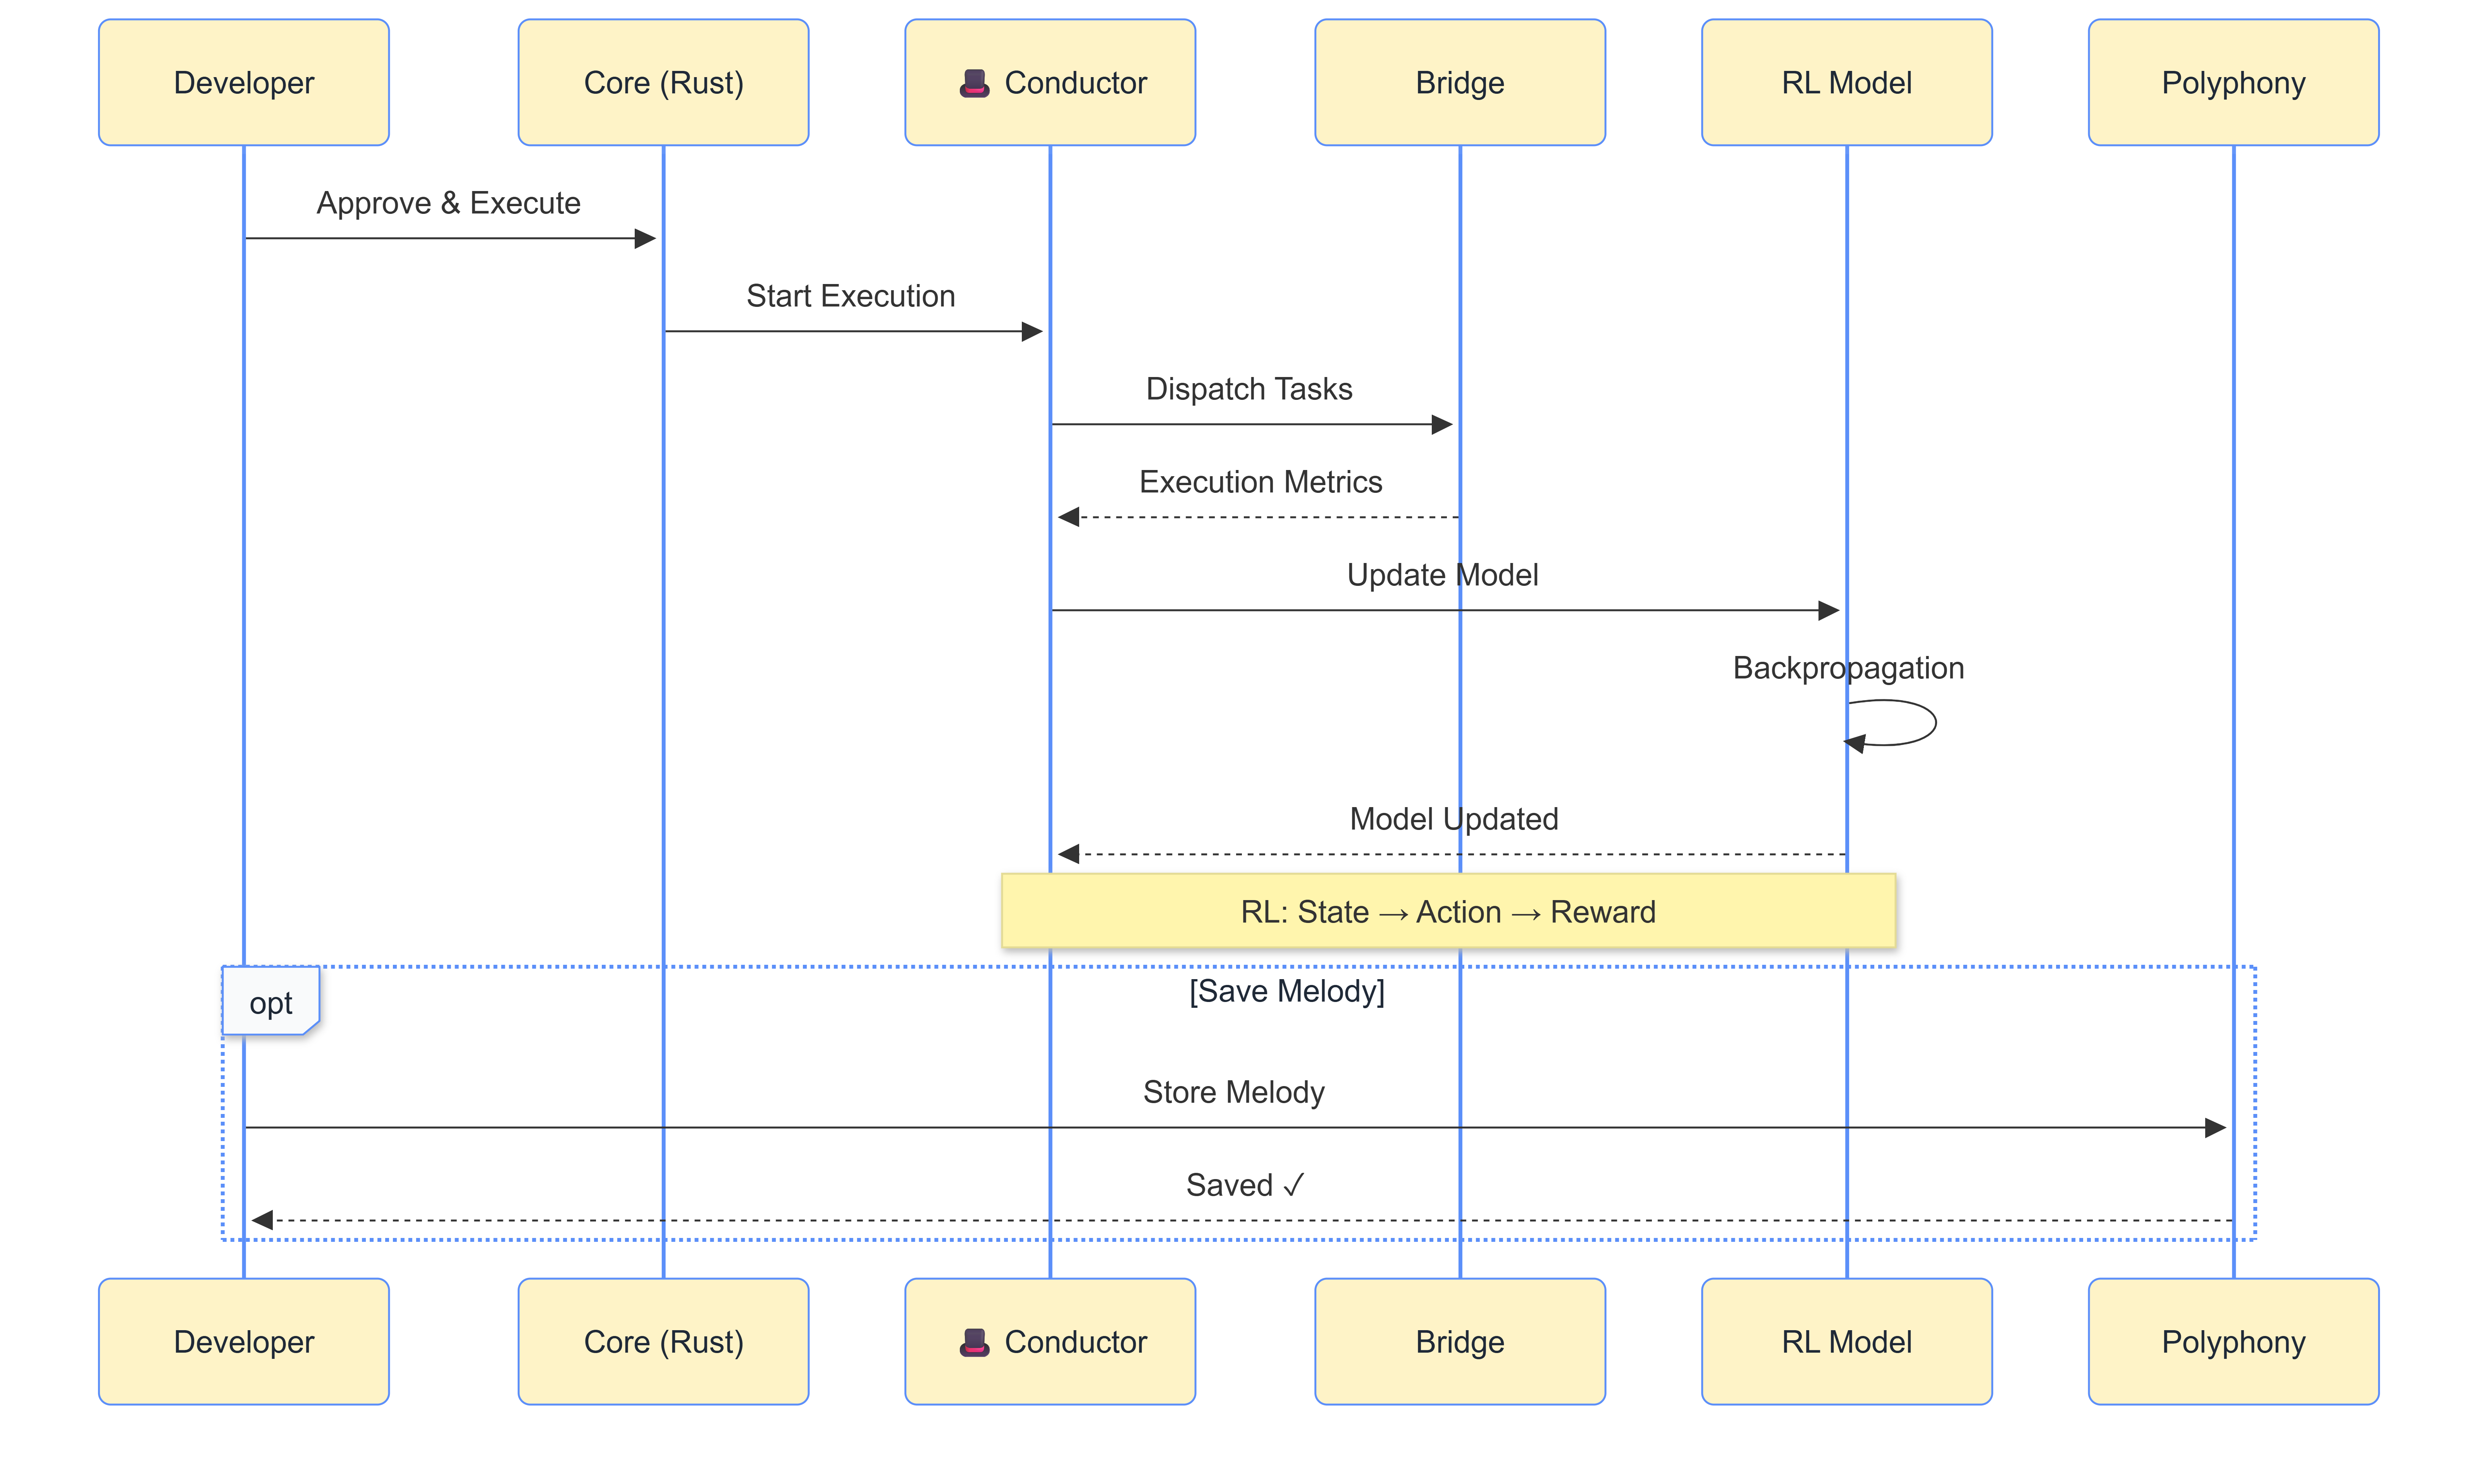
\includegraphics[width=0.95\textwidth]{images/diagrams/sequence_diagram/seperate_4_conductor_workflow_generate_melody/Execution & Learning.png}
\caption{Conductor Execution \& Learning Phase}
\label{fig:3.23-conductor-learning}
\end{figure}

% \clearpage
\subsection*{3.8.3 Workflow Execution and Validation}
\addcontentsline{toc}{subsection}{3.8.3 Workflow Execution and Validation}

The Melody execution lifecycle follows a well-defined state machine governing progression from workflow creation through completion as illustrated in ~\ref{fig:3.24-melody-states}. Melodies begin in the Draft state during composition, move through Validating for correctness checks (cycle detection, type safety, resource constraints), then Ready when validation passes. During execution, Melodies progress through Queued (waiting for resources), Executing (active processing), and optionally Paused (for checkpointing or intervention), concluding in either Completed or Failed states.

\begin{figure}[H]
\centering
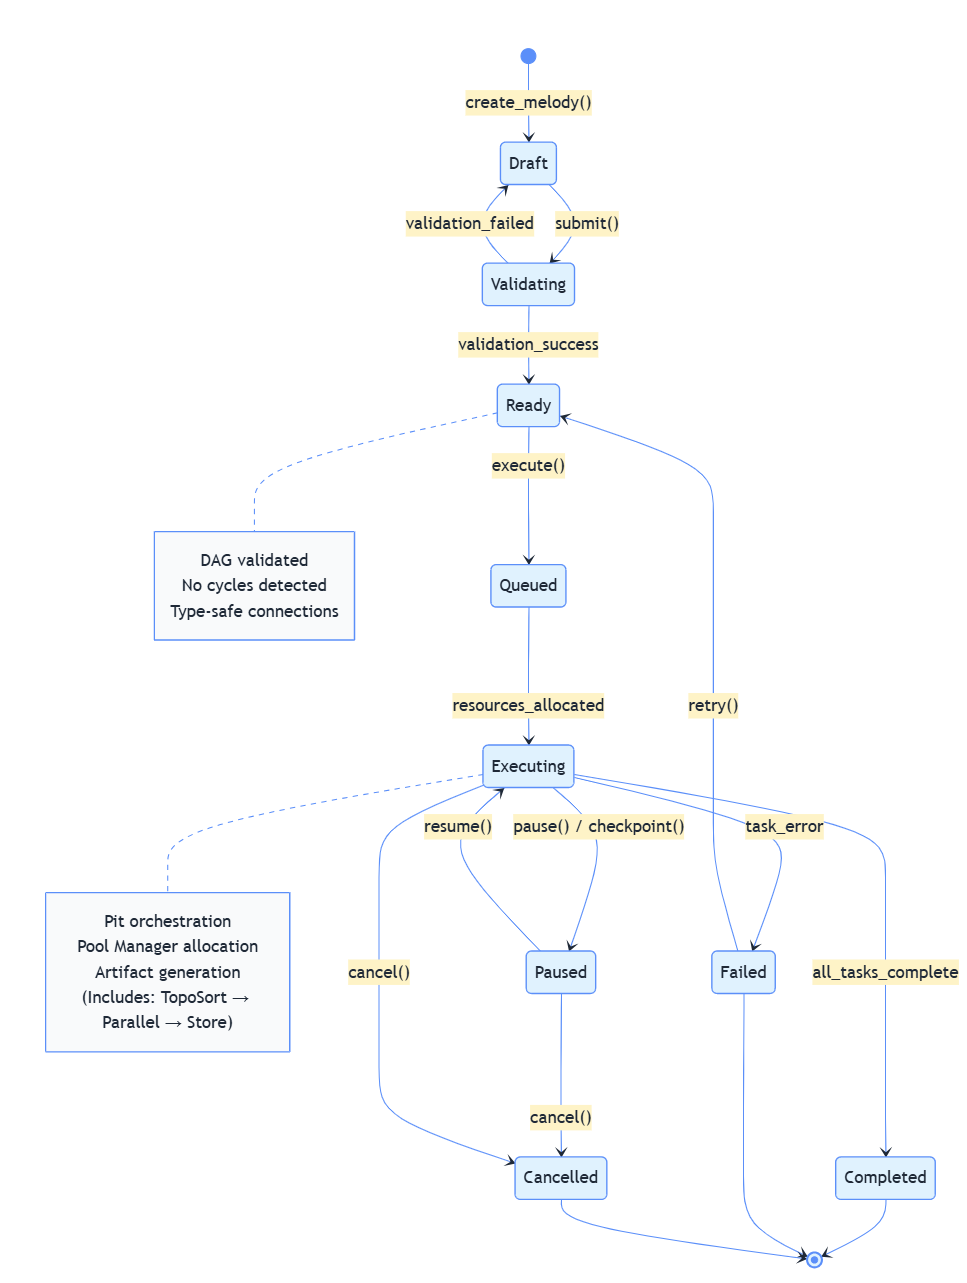
\includegraphics[width=1.05\textwidth]{images/diagrams/state_diagram/3_melody_execution_workflow.png}
\caption{Melody Execution State Machine}
\label{fig:3.24-melody-states}
\end{figure}

The orchestration system supports multiple execution modes: Maestro Mode for fully automated workflow generation from natural language prompts, Manual Mode for browsing and selecting pre-built Melodies from the Polyphony Store, and Hybrid approaches combining automated generation with manual refinement.

The workflow validation process ensures correctness before execution through cycle detection (ensuring acyclic graphs), type safety verification (compatible data flow), resource constraint validation (available resources), and dependency resolution (installed extensions). The DAG Tracker enables parallel execution by identifying independent tasks that can run concurrently, maximizing computational resource utilization while managing allocation and error handling.

Checkpoint and resume capabilities enable long-running workflows to survive system restarts by periodically saving execution state (completed tasks, outputs, remaining work). If interrupted, the system resumes from the most recent checkpoint, re-executing only incomplete tasks.

The Agent-Driven Development paradigm enabled by the orchestration system represents a fundamental shift where developers provide high-level intent while AI agents handle implementation details. This reduces cognitive load, increases productivity through automation, improves consistency by applying proven patterns, and enables exploration of different approaches.



% Section 3.6: Data Flow and System Integration
% Section 3.8: Data Flow and System Integration

\section{3.8 Data Flow and System Integration}
\label{sec:data-flow}
\addcontentsline{toc}{section}{3.8 Data Flow and System Integration}

\lettrine{T}{his section} examines how information flows through Symphony's architecture and how components integrate to form a cohesive system. We explore the directed acyclic graph model for workflow dependencies, the integration patterns that enable component collaboration, and the data governance mechanisms that ensure security and consistency. The data flow architecture provides the foundation for coordinating complex multi-step processes while maintaining clarity about data provenance and transformations.

\subsection*{3.8.1 Data Flow Model and Workflow Dependencies}
\addcontentsline{toc}{subsection}{3.8.1 Data Flow Model and Workflow Dependencies}

\lettrine{T}{he} data flow architecture of Symphony orchestrates the movement of information between components, ensuring that data reaches the right destinations at the right times while maintaining consistency and enabling efficient processing. The system treats data flow as a first-class concern, with explicit representations of how information moves through workflows and well-defined interfaces that govern data exchange between components. This architectural approach enables Symphony to coordinate complex multi-step processes involving numerous components while maintaining clarity about data provenance, transformations, and dependencies.

The conceptual data flow model represents workflows as directed acyclic graphs where nodes represent computational tasks and edges represent data dependencies between tasks. This graph-based representation makes explicit the flow of information through the system, enabling both automated reasoning about execution order and visual presentation that helps developers understand workflow structure. Each edge in the graph carries typed data, with the type system ensuring that data produced by one task is compatible with the expectations of tasks that consume it. This type safety prevents many common errors and enables early detection of incompatibilities before execution begins.

The workflow dependency management system analyzes the directed acyclic graph structure to determine valid execution orders that respect all dependencies. The topological sorting algorithm identifies a sequence in which tasks can execute such that each task runs only after all tasks it depends on have completed. When multiple valid execution orders exist, the system considers factors such as resource availability, task priorities, and opportunities for parallel execution to select an optimal order. This intelligent scheduling ensures that workflows execute efficiently while respecting all constraints and dependencies.

The overall system activity involves multiple components coordinating to process developer requests and generate outputs. The activity begins when a developer submits a prompt or selects a workflow to execute. The system analyzes the request to understand intent and identify required capabilities. The orchestration system generates or retrieves a workflow that accomplishes the objective. The execution engine processes the workflow, coordinating multiple extensions and managing data flow between them. Throughout execution, the system monitors progress, handles errors, and provides feedback to the developer. When execution completes, the system stores generated artifacts and updates its models based on the outcome. As illustrated in Figure 3.13, this complete activity flow demonstrates the coordination between all system components.

\begin{figure}[H]
\centering
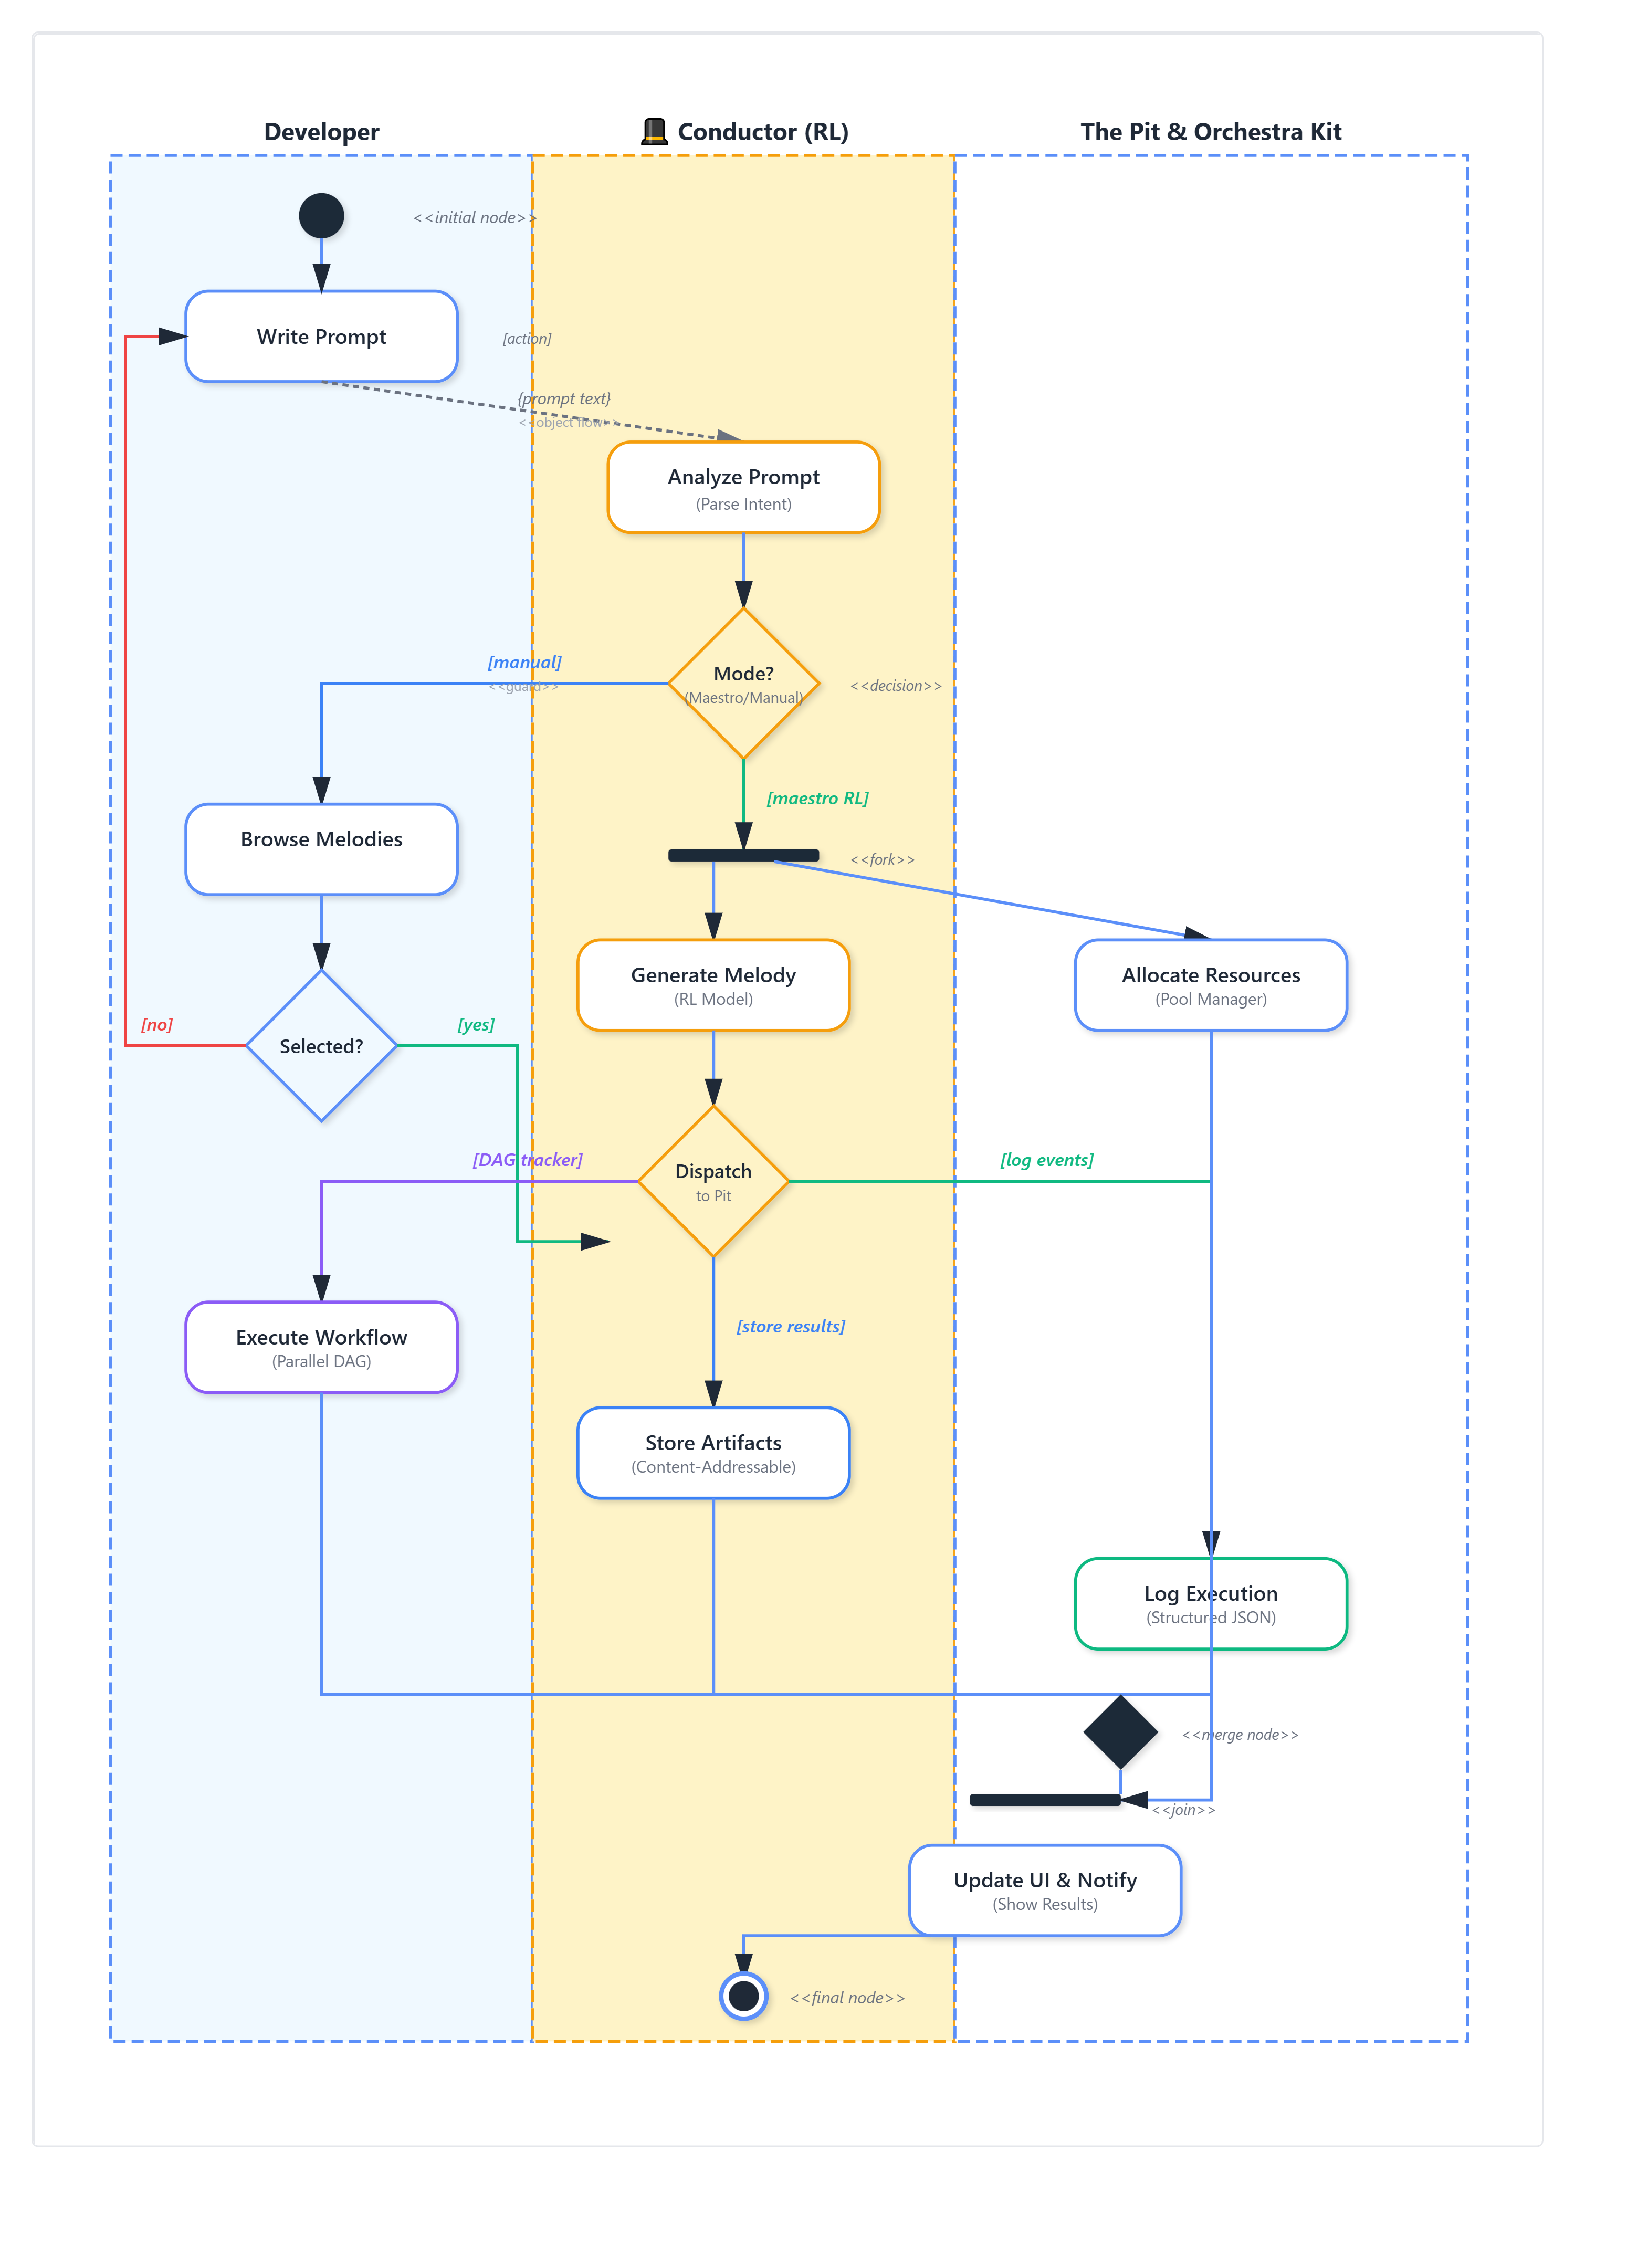
\includegraphics[width=0.95\textwidth]{images/diagrams/activity_diagram/symphony-activity-diagram.png}
\caption{Overall System Activity}
\label{fig:3.13-system-activity}
\end{figure}

\subsection*{3.8.2 Integration Patterns and Component Communication}
\addcontentsline{toc}{subsection}{3.8.2 Integration Patterns and Component Communication}

The integration patterns employed by Symphony enable components to work together effectively despite being developed independently and potentially using different technologies. The system defines clear interface contracts that specify how components communicate, what data formats they use, and what guarantees they provide. Components interact through these well-defined interfaces rather than depending on implementation details, enabling components to evolve independently as long as they continue to satisfy their interface contracts. This loose coupling between components facilitates system evolution and enables the extension ecosystem to grow without requiring coordination between extension developers.

The message passing infrastructure provides the foundation for component communication, implementing reliable delivery of messages between components regardless of whether they execute in the same process or in separate processes. The infrastructure handles serialization of complex data structures into formats suitable for transmission, routing of messages to appropriate destinations based on addressing information, buffering of messages when recipients are temporarily unavailable, and error handling when communication failures occur. This infrastructure abstracts away the complexities of inter-component communication, enabling components to focus on their domain logic rather than communication mechanics.

The data transformation capabilities enable components to work together even when they produce and consume data in different formats. The system provides a library of common transformations that convert between different representations, such as converting between different text encodings, transforming between different data structure formats, and adapting between different API conventions. Extensions can register custom transformations that handle domain-specific conversions, enabling seamless integration of specialized components. The transformation system applies conversions automatically when needed, making format differences transparent to workflow authors.

The system coordination principles that guide Symphony's integration architecture emphasize autonomy, loose coupling, and explicit contracts. Components should be autonomous, able to function independently without requiring tight coordination with other components. Components should be loosely coupled, depending on abstract interfaces rather than concrete implementations. Components should have explicit contracts that clearly specify their capabilities, requirements, and guarantees. These principles enable the system to scale to large numbers of components while maintaining understandability and reliability.

The event-driven architecture employed by Symphony enables components to react to system events without requiring tight coupling between event producers and consumers. Components can publish events to announce that interesting conditions have occurred, and other components can subscribe to events they care about without the publisher needing to know about subscribers. This publish-subscribe pattern enables flexible composition of behaviors, as new components can be added that react to existing events without modifying event publishers. The event system supports filtering and transformation, enabling subscribers to receive only relevant events in convenient formats.

The resource management system coordinates access to shared resources such as computational capacity, memory, storage, and external services. The system tracks resource availability and usage, enforces limits to prevent any component from monopolizing resources, implements fair allocation policies that ensure all components can make progress, and provides feedback to components about resource availability to enable adaptive behavior. This resource management ensures that the system remains responsive even under heavy load and that resources are allocated efficiently to maximize overall throughput.

\subsection*{3.8.3 Data Consistency and System Reliability}
\addcontentsline{toc}{subsection}{3.8.3 Data Consistency and System Reliability}

The error handling and recovery mechanisms ensure that the system remains stable and functional even when individual components encounter errors. The system implements fault isolation to prevent errors in one component from affecting others, automatic retry with exponential backoff for transient failures, graceful degradation when components become unavailable, and comprehensive logging to facilitate debugging and root cause analysis. These mechanisms ensure that Symphony provides a reliable platform for development even when dealing with the inherent unreliability of complex distributed systems.

The data consistency mechanisms ensure that information remains accurate and coherent as it flows through the system. The system implements transactional semantics for operations that must complete atomically, optimistic concurrency control for operations that rarely conflict, eventual consistency for operations where immediate consistency is not required, and conflict resolution strategies for situations where concurrent updates create inconsistencies. These mechanisms provide appropriate consistency guarantees for different types of operations while enabling high performance and availability.

The caching strategies employed throughout the system reduce latency and improve throughput by avoiding redundant computation and data retrieval. The system caches frequently accessed data close to where it is used, invalidates cached data when underlying sources change, implements cache warming to preload data that is likely to be needed, and applies eviction policies to manage cache size when memory is limited. These caching strategies significantly improve system responsiveness while ensuring that cached data remains accurate.

The monitoring and observability capabilities enable developers and system administrators to understand system behavior and diagnose issues. The system collects metrics about component performance, resource usage, error rates, and other operational characteristics. These metrics are aggregated and made available through dashboards and APIs that enable real-time monitoring and historical analysis. The system also implements distributed tracing that tracks requests as they flow through multiple components, enabling developers to understand the complete path of execution and identify bottlenecks or errors.

The integration testing framework enables verification that components work together correctly despite being developed independently. The framework provides tools for setting up test environments that include multiple components, generating test data that exercises integration points, asserting expected behaviors and outcomes, and cleaning up test environments after tests complete. This testing capability ensures that integration issues are caught early in the development process rather than manifesting as production failures.

The versioning and compatibility management system enables the extension ecosystem to evolve while maintaining stability for existing workflows. The system uses semantic versioning to communicate the nature of changes in new extension versions, maintains multiple versions of extensions to support workflows that depend on specific versions, provides compatibility shims that enable old workflows to work with new extension versions, and validates that workflow dependencies can be satisfied before execution begins. This versioning approach enables innovation while protecting existing workflows from breaking changes.

The data governance policies ensure that sensitive information is handled appropriately as it flows through the system. The system implements access controls that restrict which components can access sensitive data, audit logging that records all access to sensitive information, encryption for data at rest and in transit, and data retention policies that ensure information is not kept longer than necessary. These governance mechanisms enable Symphony to be used in environments with strict data handling requirements while maintaining the flexibility and power of the extension ecosystem.


% Section 3.7: User Interface Design Principles
% Section 3.9: User Interface Design Principles

\section{3.9 User Interface Design Principles}
\label{sec:ui-design}
\addcontentsline{toc}{section}{3.9 User Interface Design Principles}

\lettrine{T}{his section} explores Symphony's user interface design philosophy and the interaction paradigms that enable effective human-AI collaboration. We examine the visual workflow composition system, real-time feedback mechanisms, and accessibility features that make Symphony both powerful and approachable. The interface design emphasizes clarity of intent, progressive disclosure, and multi-modal interaction to support diverse development scenarios and user preferences.

\subsection*{3.9.1 AI-First Interaction Paradigm and Visual Composition}
\addcontentsline{toc}{subsection}{3.9.1 AI-First Interaction Paradigm and Visual Composition}

\lettrine{T}{he} user interface design of Symphony embodies a fundamental rethinking of how developers interact with AI-powered development environments. The design philosophy recognizes that traditional code-centric interfaces are insufficient for environments where AI agents handle much of the implementation work, and that new interaction paradigms are needed to enable effective human-AI collaboration. The interface design emphasizes clarity of intent over precision of instruction, visual representation of complex workflows over textual descriptions, and real-time feedback about AI activities over passive waiting for results.

The AI-first interaction paradigm shifts the developer's role from writing detailed instructions to providing high-level guidance and making strategic decisions. The interface supports this paradigm shift by providing mechanisms for expressing intent through natural language prompts, visualizing how the system interprets and plans to execute those intents, enabling developers to review and refine automatically generated plans before execution, and providing comprehensive visibility into AI activities during execution. This interaction model reduces cognitive load by eliminating the need to specify every detail while maintaining developer control through review and approval mechanisms.

The visual workflow composition capabilities provided by the Harmony Board enable developers to create and understand complex workflows through direct manipulation rather than textual programming. The interface presents workflows as node-and-edge graphs where nodes represent individual tasks and edges represent data dependencies. Developers can drag nodes from a palette onto the canvas to add tasks, draw edges between nodes to establish dependencies, configure node parameters through property panels, and arrange the layout to improve clarity. This visual approach makes workflow structure immediately apparent and enables developers to reason about complex processes more effectively than textual representations would allow.

The Harmony Board creation process involves multiple steps that guide developers from initial concept to executable workflow. The process begins with opening the Harmony Board in creation mode and loading the palette of available extensions. Developers drag nodes representing Instruments, Operators, and Motifs onto the canvas to build the workflow structure. The system validates connections in real-time as developers draw edges between nodes, providing immediate feedback about type compatibility and other constraints. Developers configure parameters for each node, specifying inputs, resource limits, and other settings. The system validates the complete workflow to ensure it forms a valid directed acyclic graph with no cycles or type mismatches. Once validation passes, developers can save the workflow to the Polyphony Store and optionally publish it for others to use. As illustrated in Figure 3.14, this complete creation process demonstrates the visual workflow composition capabilities.

\begin{figure}[H]
\centering
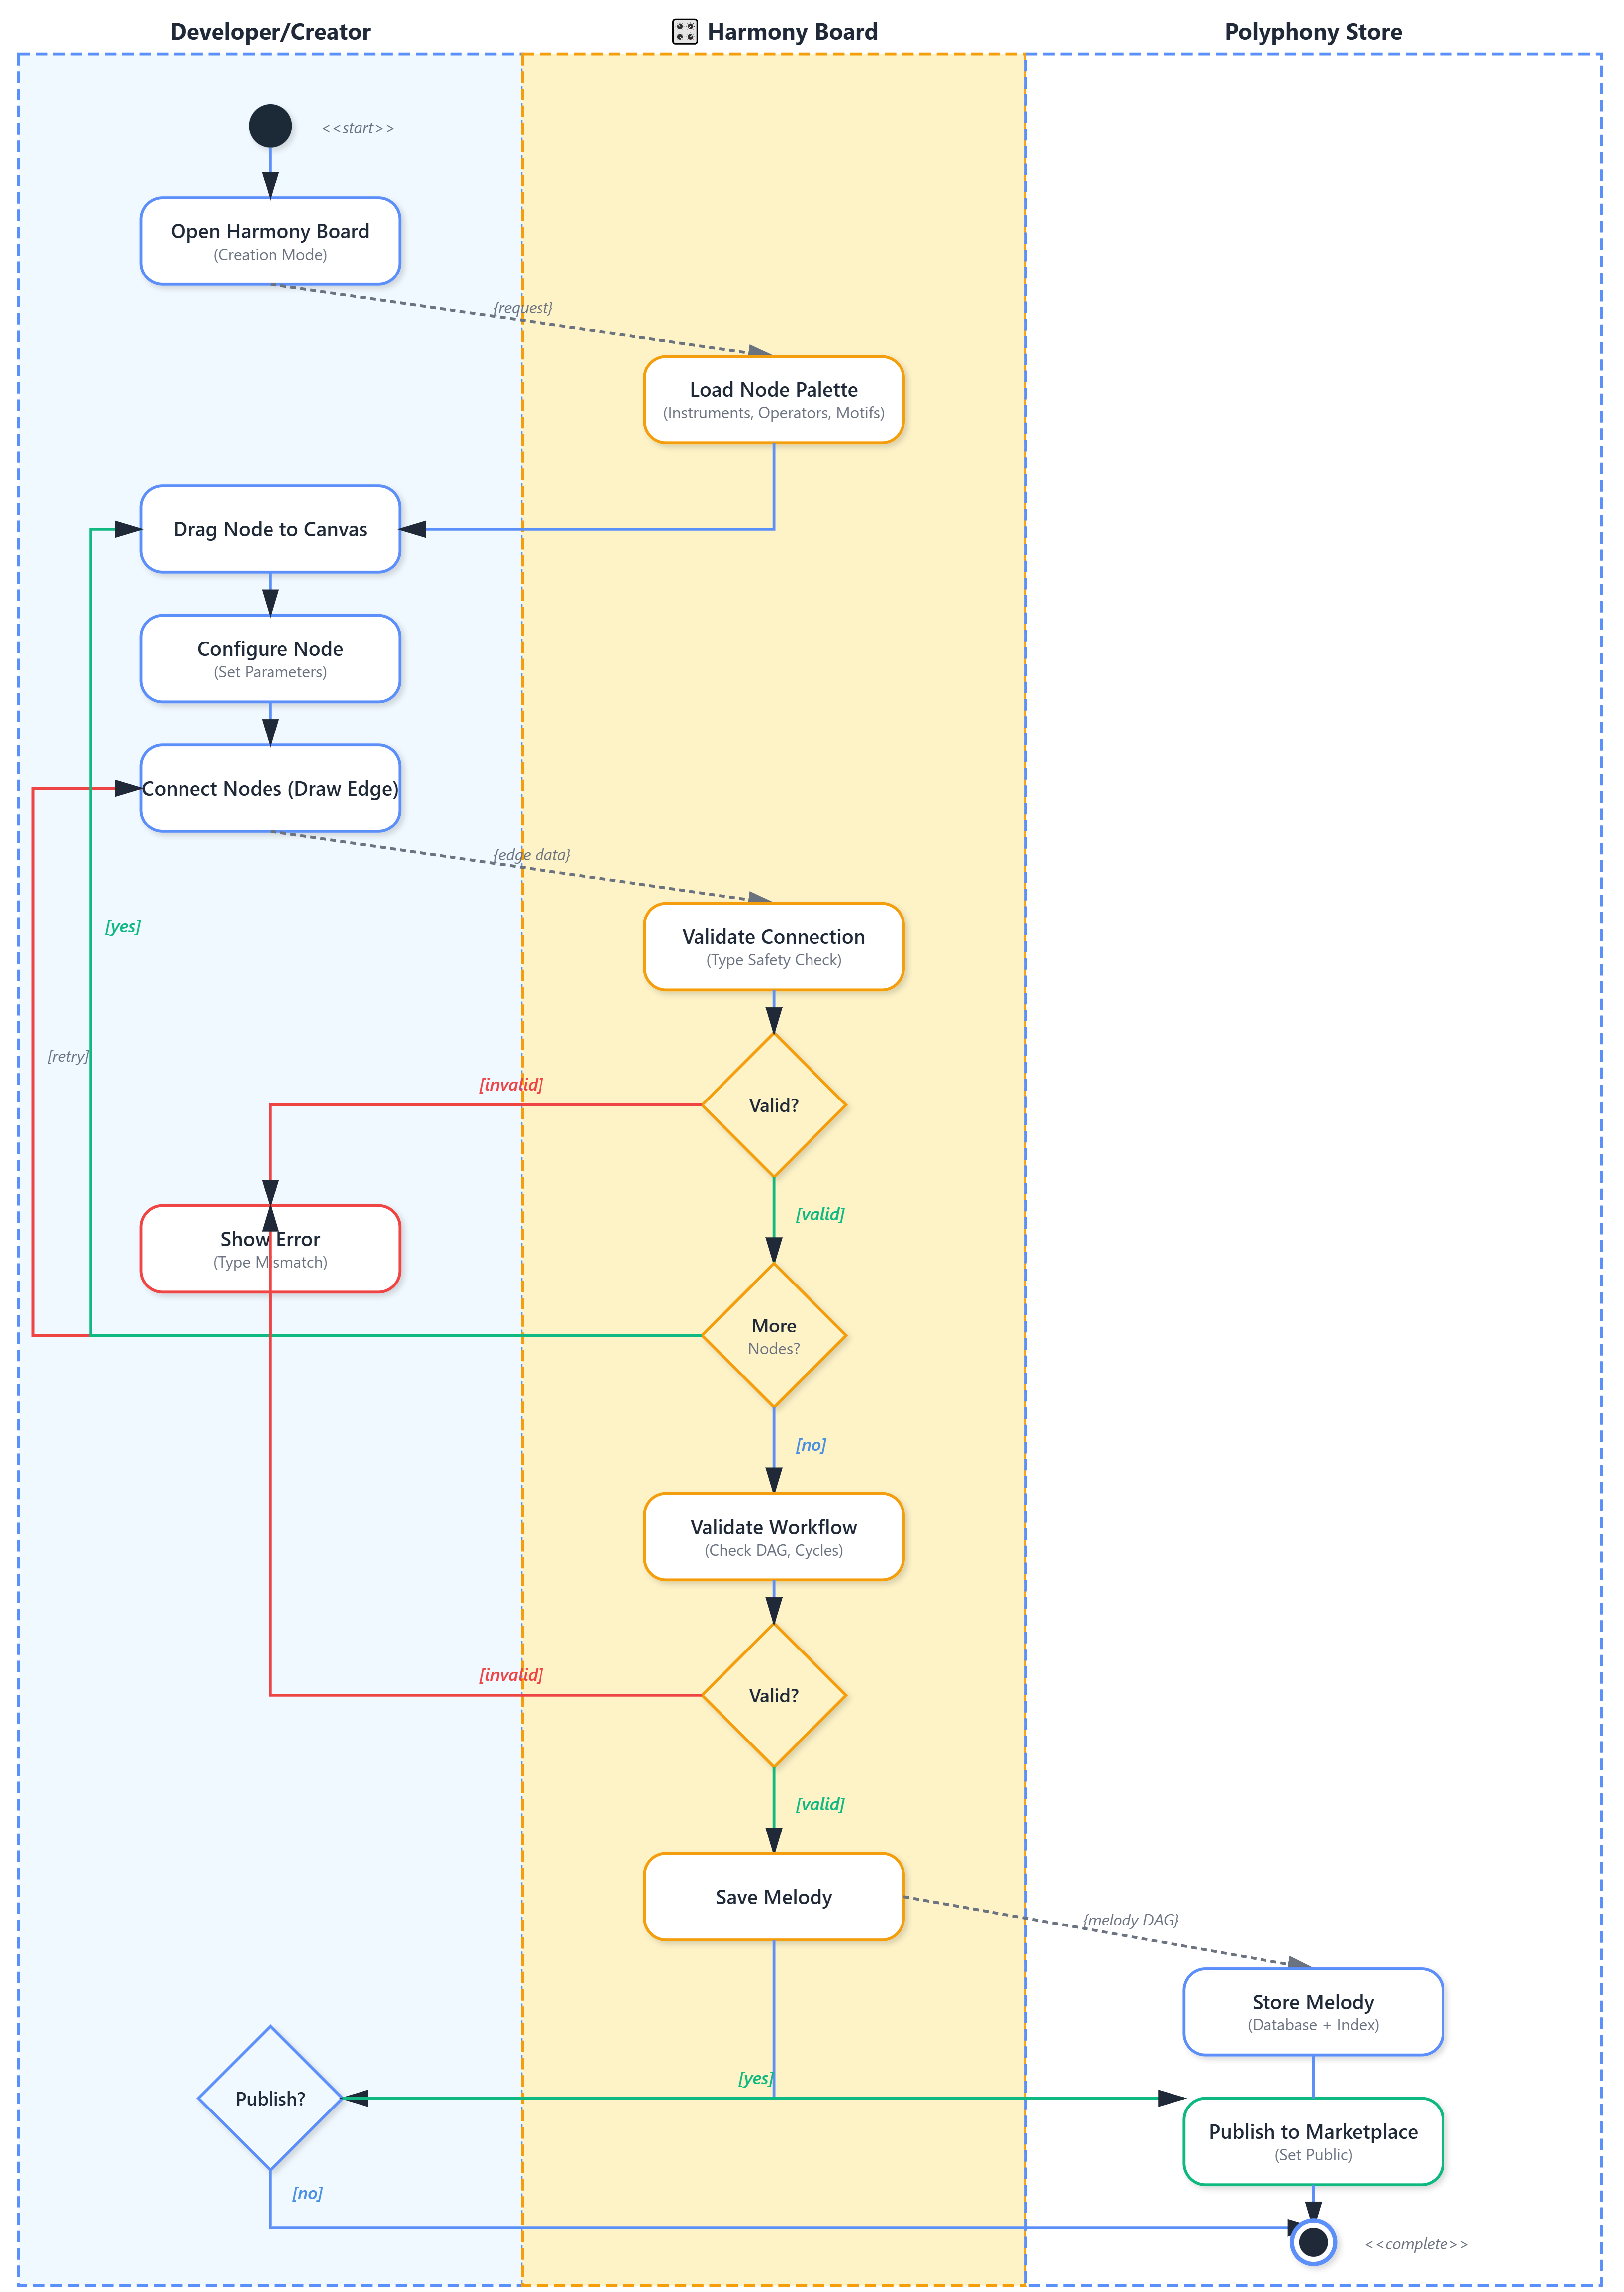
\includegraphics[width=0.95\textwidth]{images/diagrams/activity_diagram/symphony-harmony-board-creation.png}
\caption{Harmony Board Creation Process}
\label{fig:3.14-harmony-board-creation}
\end{figure}

\subsection*{3.9.2 Feedback, Context Awareness, and User Experience}
\addcontentsline{toc}{subsection}{3.9.2 Feedback, Context Awareness, and User Experience}

The real-time feedback mechanisms keep developers informed about AI activities through progress indicators showing task execution status, completion percentage, and estimated time remaining. The interface highlights errors immediately with stack traces and diagnostic information, building trust through transparency. Context-aware assistance adapts based on current development context, suggesting relevant workflows and highlighting applicable extensions to reduce cognitive burden.

The progressive disclosure approach manages complexity by showing essential information by default while making advanced details available on demand. Multi-modal interaction enables developers to use natural language prompts, visual workflow composition, direct code editing, or voice commands based on task requirements and preferences. Collaborative features support real-time multi-developer workflows with change tracking, attribution, and workflow sharing through the Polyphony Store.

Accessibility considerations ensure broad usability through keyboard navigation, screen reader compatibility, customizable color schemes including high-contrast modes, and adjustable font sizes for diverse developer abilities and preferences.

\subsection*{3.9.3 System Integration and User Empowerment}
\addcontentsline{toc}{subsection}{3.9.3 System Integration and User Empowerment}

Performance optimization ensures responsive interface through virtual scrolling, lazy loading, incremental rendering, and background processing. Error presentation shows issues in context with suggested fixes and quick actions for retry or rollback. Workspace management enables independent configuration of multiple environments with different extensions, settings, and workflows for different projects or contexts.

Customization capabilities support custom color themes, keyboard shortcuts, layouts, and extensions to match individual preferences. Integration with external tools displays information from issue trackers, version control, and CI services, enabling Symphony to complement existing development infrastructure. Performance monitoring provides execution time, resource utilization, bottleneck identification, and historical trends for workflow optimization.

The design principles emphasize clarity through understandable system behavior, efficiency through minimized steps for common tasks, and empowerment by giving developers control over AI activities while reducing routine task burden. These principles ensure that Symphony's interface serves developers effectively while supporting the AI-first development paradigm. As shown in Figure 3.15, the diverse use cases demonstrate the system's flexibility and breadth of functionality.

\begin{figure}[H]
\centering
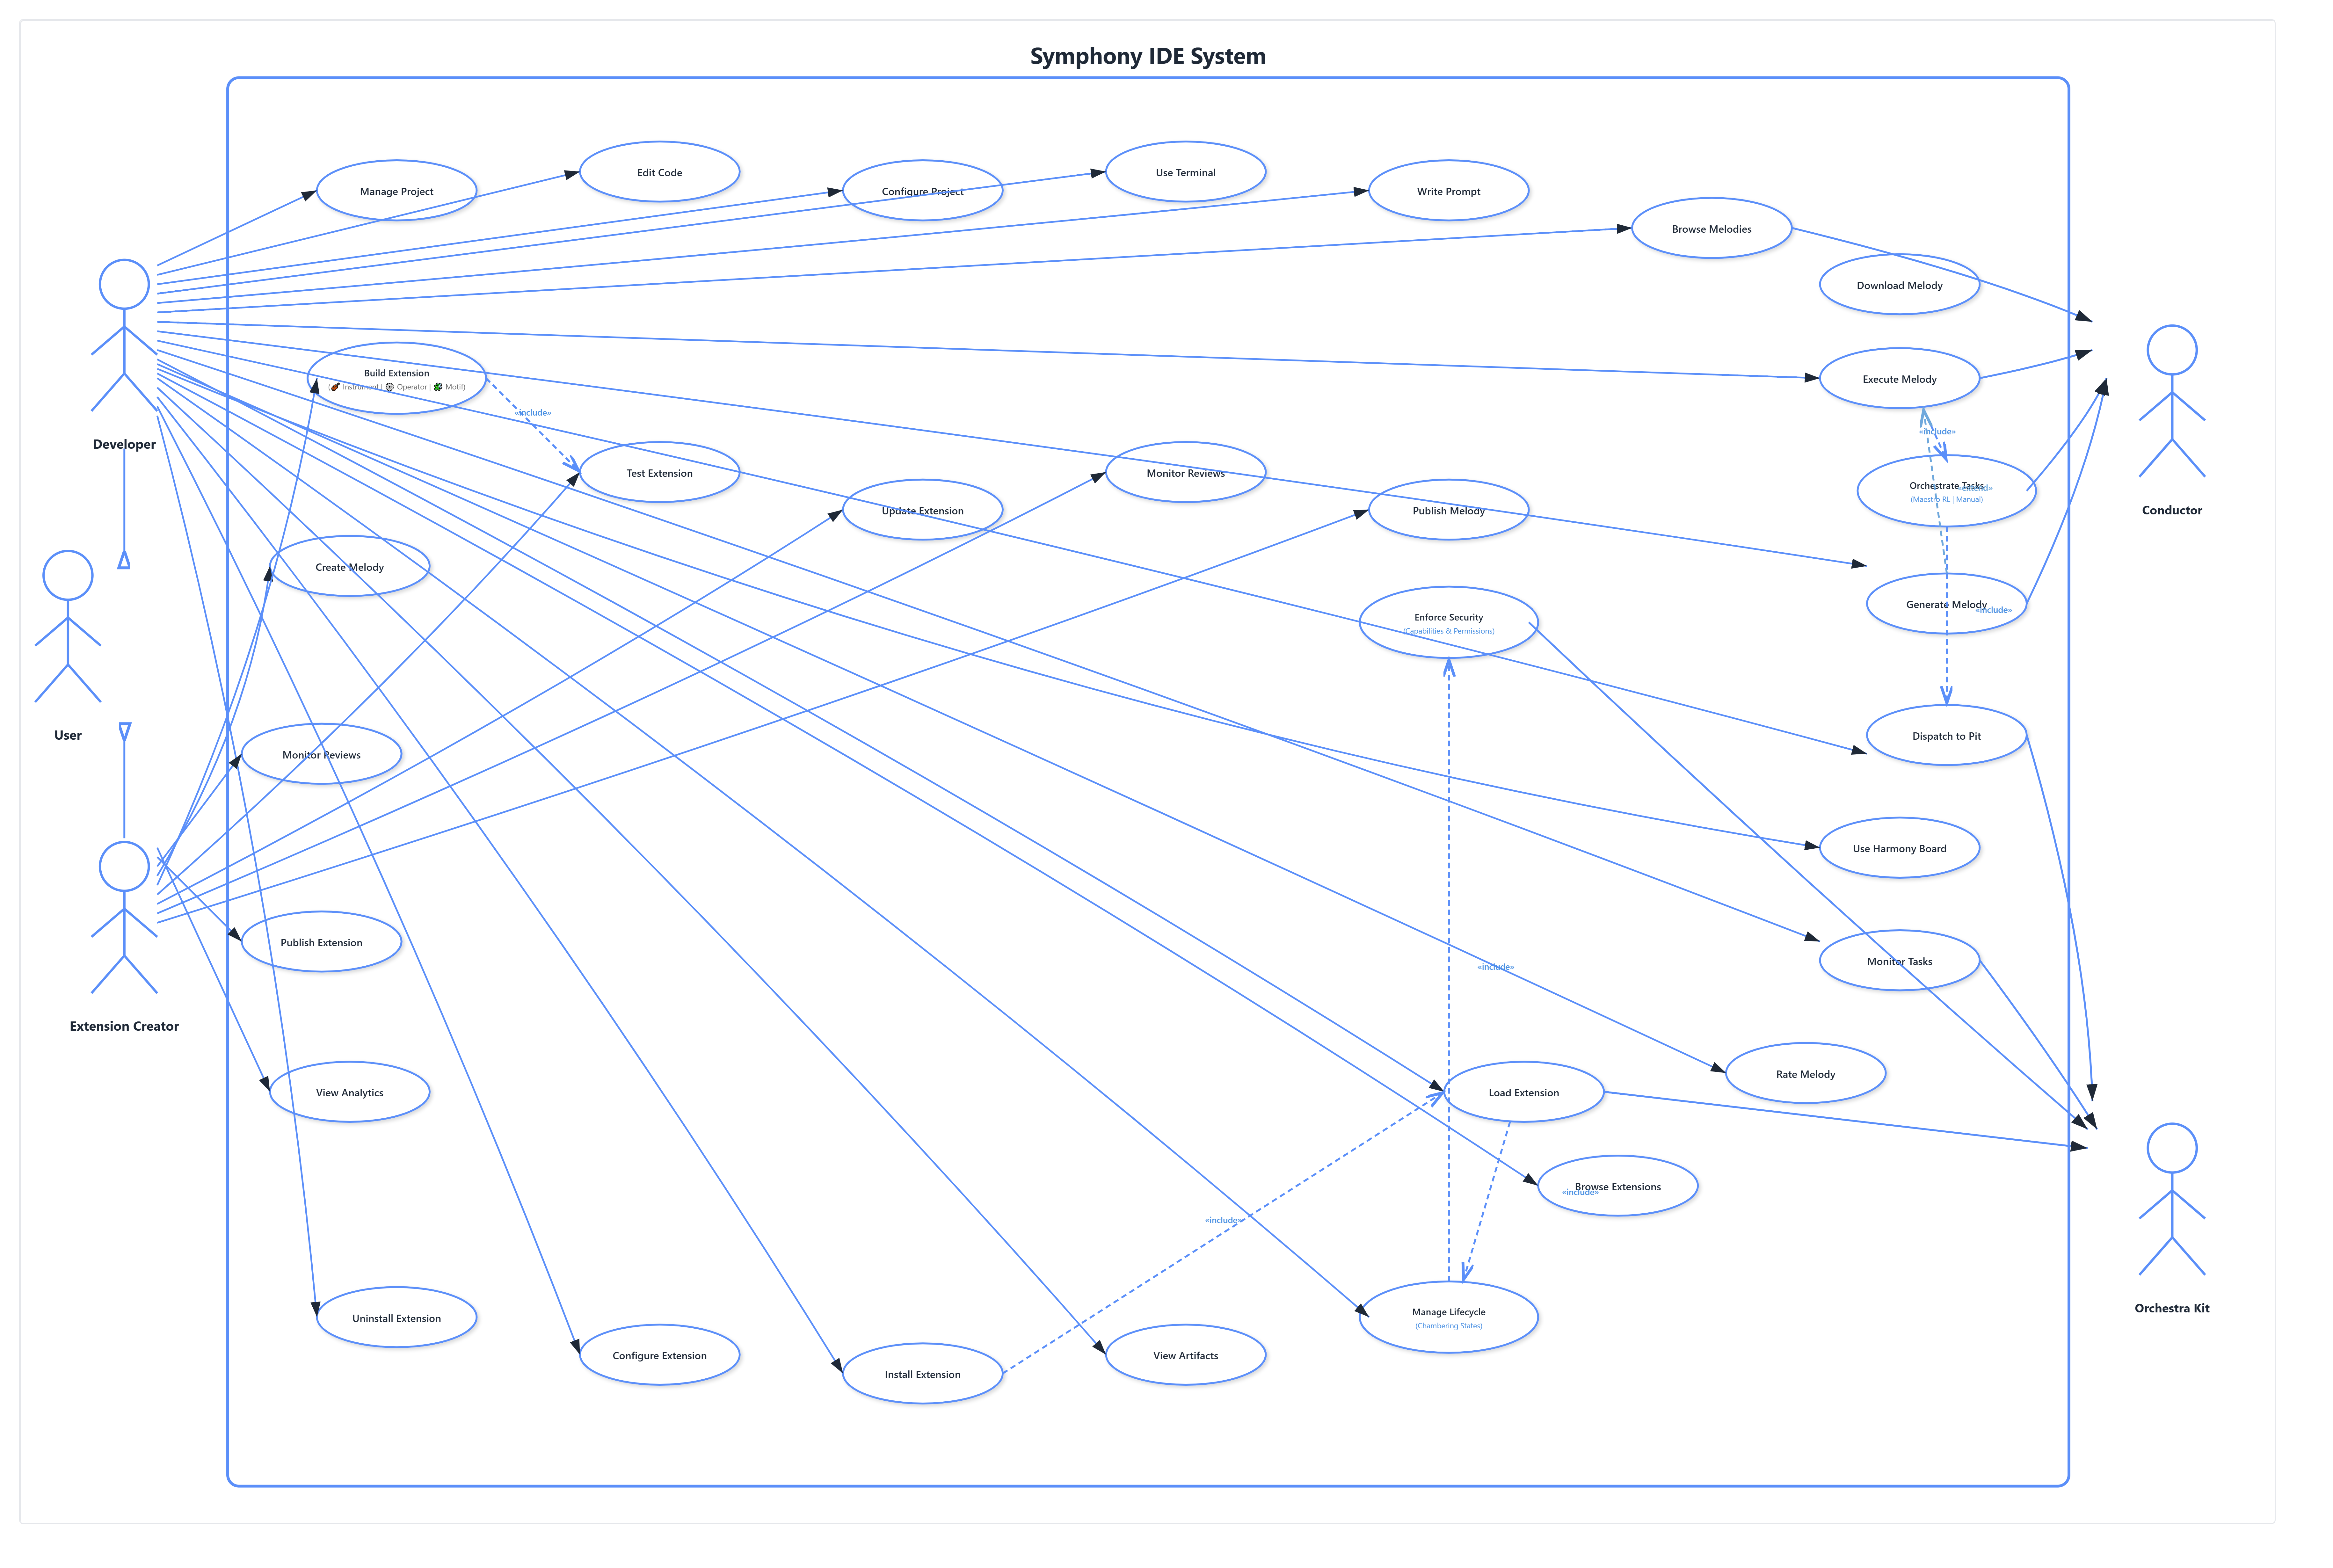
\includegraphics[width=0.85\textwidth]{images/diagrams/use-case.png}
\caption{System Use Cases}
\label{fig:3.15-use-cases}
\end{figure}


% Section 3.8: Generic Primitives and Protocol Support
% % Section 3.8: Generic Primitives and Protocol Support

\section{3.8 Generic Primitives and Protocol Support}
\label{sec:generic-primitives}

\lettrine{S}{ymphony's} approach to protocol support represents a fundamental departure from traditional development environments. Rather than hardcoding support for specific protocols such as Language Server Protocol or Debug Adapter Protocol, Symphony provides generic communication and data handling primitives that can adapt to any protocol. This protocol-agnostic design ensures future-proof extensibility and enables community-driven innovation without requiring core system modifications.

\subsection*{No Hardcoded Protocols Philosophy}

Traditional development environments often embed protocol support directly into their core architecture, creating several limitations: version lock-in requiring core updates when protocols evolve, limited innovation where new protocols require vendor approval and core modifications, bloated core where each supported protocol adds complexity and maintenance burden, and rigid assumptions where protocol-specific optimizations may not suit all use cases.

Symphony eliminates these limitations by providing generic primitives that extensions compose to implement whatever communication patterns they need. This composition-over-configuration approach enables extensions to support any protocol without core system changes.

\begin{table}[H]
\caption{Protocol Support: Traditional vs Generic Approaches}
\centering
\begin{tabular}{@{}p{0.45\textwidth}p{0.45\textwidth}@{}}
\toprule
\textbf{Traditional Approach} & \textbf{Symphony's Generic Primitives} \\
\midrule
Hardcoded LSP support & Generic JSON-RPC communication \\
Built-in DAP integration & Flexible process communication \\
Specific Git commands & Generic subprocess management \\
Fixed protocol versions & Version-agnostic message handling \\
Vendor-controlled updates & Community-driven protocol evolution \\
\bottomrule
\end{tabular}
\end{table}

\subsection*{Message Format Abstraction}

Symphony supports multiple message formats through a unified interface, enabling extensions to choose the most appropriate serialization for their needs:

\begin{compactlist}
    \item \textbf{JSON}: Standard JSON-RPC and custom JSON protocols
    \item \textbf{MessagePack}: Binary serialization for performance-critical applications
    \item \textbf{Protocol Buffers}: Strongly-typed binary protocols
    \item \textbf{Plain Text}: Simple line-based or custom text protocols
    \item \textbf{Custom Formats}: Extensions can implement their own serialization
\end{compactlist}

\subsection*{Transport Layer Abstraction}

The transport layer provides multiple communication mechanisms enabling extensions to select optimal transport based on their specific requirements:

\begin{compactlist}
    \item \textbf{Standard I/O}: Process stdin/stdout communication
    \item \textbf{TCP Sockets}: Network-based communication
    \item \textbf{WebSockets}: Real-time bidirectional communication
    \item \textbf{Named Pipes}: High-performance local communication
    \item \textbf{HTTP/REST}: Request-response web protocols
\end{compactlist}

\subsection*{Capability Negotiation and Discovery}

Symphony's generic primitives include sophisticated capability negotiation allowing extensions and external tools to discover each other's capabilities dynamically. When an extension connects to an external tool, Symphony facilitates automatic negotiation of message formats, transport mechanisms, and protocol versions, ensuring optimal communication without requiring manual configuration.

The negotiation process follows these steps: capability advertisement where each party advertises supported formats and transports, preference matching where Symphony finds the optimal combination based on performance and compatibility, fallback handling with graceful degradation to simpler formats if needed, and dynamic adaptation with runtime switching if conditions change.

\subsection*{UI Extensibility Framework}

Symphony's UI extensibility framework allows extensions to create custom user interfaces while maintaining consistency and performance. The framework provides four levels of customization:

\begin{table}[H]
\caption{UI Extensibility Levels and Capabilities}
\centering
\begin{tabular}{@{}p{0.3\textwidth}p{0.35\textwidth}p{0.3\textwidth}@{}}
\toprule
\textbf{Customization Level} & \textbf{Capabilities} & \textbf{Use Cases} \\
\midrule
\textbf{Component Registration} & 
Custom React components, event handlers, styling & 
Status bars, toolbars, buttons \\
\midrule
\textbf{View Creation} & 
Full custom views, data binding, lifecycle management & 
File explorers, output panels, search results \\
\midrule
\textbf{Layout Modification} & 
Panel arrangement, window management, workspace organization & 
IDE layouts, multi-pane editors, dashboards \\
\midrule
\textbf{Virtual DOM Bridge} & 
Direct DOM manipulation, custom rendering, performance optimization & 
Complex visualizations, real-time displays \\
\bottomrule
\end{tabular}
\end{table}

The UI framework defines several extensible regions including Editor Area for central editing space with tab management, Sidebar Panels for left and right collapsible panels, Bottom Panel for terminal and output, Top Toolbar for action buttons and menu integration, Status Bar for information and quick actions, and Modal Overlays for dialogs and command palette.

Extensions can create and manage panels dynamically, with automatic theming ensuring extension UIs adapt to user-selected themes, responsive layout where components automatically adjust to window size changes, performance optimization through virtual DOM and efficient rendering, accessibility with built-in keyboard navigation and screen reader support, and consistency through shared design system ensuring cohesive user experience.

\subsection*{Benefits of Generic Primitives Approach}

This protocol-agnostic architecture provides several key advantages:

\begin{compactlist}
    \item \textbf{Future-Proof}: New protocols can be supported without core changes
    \item \textbf{Innovation-Friendly}: Community can experiment with novel communication patterns
    \item \textbf{Lightweight Core}: No protocol-specific code bloating the core system
    \item \textbf{Universal Compatibility}: Same primitives work for any external tool or service
    \item \textbf{Performance-Optimized}: Each extension can choose the most efficient transport and format
    \item \textbf{Interoperability}: Different extensions can communicate using compatible primitives
\end{compactlist}

This approach transforms Symphony from a traditional development environment into a protocol-agnostic development platform that can adapt to any workflow or toolchain through its extension ecosystem, enabling unlimited extensibility without compromising core system simplicity or performance.

